\documentclass{llncs}

\usepackage{xcolor}
\usepackage{enumitem,amsmath,amssymb}
\usepackage{stmaryrd}    % needed for \mapsfrom
\usepackage{algorithm2e}
\usepackage{bussproofs}
\def\defaultHypSeparation{\hskip.1in}

\usepackage{tikz}

\usepackage{logictools}
\usepackage{prooftheory}
\usepackage{comment}
\usepackage{mathenvironments}


\title{Propositional Resolution Proof Compression by Lowering Nodes}

\author{
  Joseph Boudou\inst{1}\thanks{This work was partly supported by the Google Summer of Code program.}
  \and 
  Bruno Woltzenlogel Paleo\inst{2}
}

\authorrunning{J.\~Boudou \and B.\~Woltzenlogel Paleo}

\institute{
  Universit\'e Paul Sabatier, Toulouse \\
  \email{joseph.boudou@matabio.net}
  \and 
  Vienna University of Technology \\
  \email{bruno@logic.at}
}





\begin{document}

\maketitle


\begin{abstract}
This paper describes a generalization of the {\LowerUnits} algorithm \cite{LURPI} for the compression
of propositional resolution proofs. The generalized algorithm, here called {\LowerUnivalents}, is
able to lower not only units but also proof nodes containing non-unit clauses, provided that their
literals satisfy some additional conditions. A formal proof that {\LowerUnivalents} always
compresses more than {\LowerUnits} is shown, and both algorithms are empirically compared on
thousands of proofs produced by the SMT-Solver \veriT.
\end{abstract}

\section{Introduction}

Sat-solvers are among the most successful automated deduction tools available today. As standalone tools, they can already be applied to a wide range of problems, especially considering that, due to the NP-completeness of propositional satisfiability \cite{cook}, any NP problem can be encoded as a propositional formula. And, nevertheless, despite the theoretical difficulty associated with NP problems, state-of-the-art sat-solving techniques perform surprisingly well in practice \cite{sat-competition}. With the aim of leveraging this efficiency, sat-solvers have been embedded into various other automated deduction tools that target problems described in more expressive logics. The most prominent examples are SMT-solvers \cite{veriT}, for checking satisfiability modulo theories for equality, linear arithmetic, bit-vectors, arrays and others. But more recently, interactive proof assistants \cite{isabelle-blanchette-boehme} and automated first-order \cite{spassT?MELIA?iProver?Vampire?} and even higher-order \cite{satallax} theorem provers have taken advantage of embedding sat-solvers too.

In such a scenario, it is essential that sat-solvers output not only a \emph{yes} or \emph{no} answer, but also a model (in case of satisfiability) or a refutation (in case of unsatisfiability). For DPLL- and CDCL-based sat-solvers, propositional resolution is an excellent proof system, since refutations in this system can be generated with an acceptable efficiency overhead and they are detailed enough to allow easy implementation of efficient proof checkers.

ToDo: unsat core, interpolants...

With the increase in the demand for proofs from sat-solvers, there has been a surge of techniques to compress and improve such proofs in a post-processing stage. ToDo: briefly describe and list related work here.

In this paper...  ToDo: modify and expand the abstract here\\
 describes a generalization of the {\LowerUnits} algorithm \cite{LURPI} for the compression
of propositional resolution proofs. The generalized algorithm, here called {\LowerUnivalents}, is
able to lower not only units but also proof nodes containing non-unit clauses, provided that their
literals satisfy some additional conditions. A formal proof that {\LowerUnivalents} always
compresses more than {\LowerUnits} is shown, and both algorithms are empirically compared on
thousands of proofs produced by the SMT-Solver \veriT.

ToDo: explain the organization of the paper here.


\section{Propositional Resolution Calculus}

A \emph{literal} is a propositional variable or the negation of a propositional variable. The \emph{dual} of a literal $\ell$ is denoted
$\dual{\ell}$ (i.e. for any propositional variable $p$, $\dual{p} =
\neg p$ and $\dual{\neg p} = p$) and the \emph{underlying variable} of a literal
$\ell$ is written $|\ell|$ (i.e. $|p| = |\neg p| = p$). The set of all literals is denoted $\mathcal{L}$. A \emph{clause} is a set of literals. $\bot$ denotes the \emph{empty clause}.


\noindent
A \emph{proof} of a clause $\Gamma$ from a set of clauses $\mathcal{A}$ is a
directed acyclic graph where: leaves contain \emph{axioms} from $\mathcal{A}$;
any inner node $\eta$ has exactly two outgoing edges to its \emph{premises} $\eta^L$ and $\eta^R$, and $\eta$'s clause is a resolvent of its premises' clauses; the edges are labeled by the premises'
resolved literals; and there is a single \emph{root} node, containing clause $\Gamma$. A \emph{refutation} of $\mathcal{A}$ is a proof of $\bot$ from $\mathcal{A}$.


\begin{definition}[Proof] \label{def:proof}
A proof is a directed acyclic graph
$\langle 
V, 
E, 
\mathcal{A},
\clause, 
\rho
\rangle$, 
where $V$ is a set of nodes, $E \subset V \times \mathcal{L} \times V$, 
$\mathcal{A} \subset 2^\mathcal{L}$,
$\clause : V \longrightarrow 2^\mathcal{L}$, 
$\rho \in V$, and such that it is inductively constructible as follows:
\begin{enumerate}
  \item $\langle \{\rho\}, \varnothing, \{ \Gamma \}, \{ (\rho, \Gamma) \}, \varnothing,  \rho \rangle$ 
    is a proof of $\Gamma$ from $\{ \Gamma \}$.
  \item If $\psi_L$ is a proof $\langle V_L, E_L, \mathcal{A}_L, \clause_L, \rho_L \rangle$ and
    $\psi_R$ is a proof $\langle V_R, E_R, \mathcal{A}_R, \clause_R, \rho_R \rangle$, then, for any $a$ such that $\dual{a} \in \clause(\rho_L)$ and $a
    \in \clause(\rho_R)$ and a new node $\rho$, the graph 
    $\langle 
    V_L \cup V_R \cup \{\rho\},
    E_L \cup E_R \cup \{\rho \xrightarrow{\dual{a}} \rho_L, \rho \xrightarrow{a} \rho_R\}, 
    \mathcal{A}_L \cup \mathcal{A}_R,
    \clause,
    \rho
    \rangle$ where
    \begin{equation*}
      \clause(\eta) = \begin{cases}
        \clause_L(\eta) & \eta \in V_L \\
        \clause_R(\eta) & \eta \in V_R \\
        (\clause_L(\rho_L) \setminus \{\dual{a}\}) \cup (\clause_R(\rho_R) \setminus \{a\}) &
          \eta = \rho
      \end{cases}
    \end{equation*}
    is a proof of $\clause(\rho)$ from $\mathcal{A}_L \cup \mathcal{A}_R$, and is denoted $\psi_L \odot_a \psi_R$.
  \qed
\end{enumerate}
\end{definition}


\BWP{ToDo: fix this paragraph} $E$ is the \emph{premise} or \emph{parent} relation. Its inverse relation is the \emph{child} relation and its
transitive closure is the \emph{ancestor} relation.  

As the premises are unordered $\psi_L \odot_a \psi_R$ denotes the same proof as $\psi_R
\odot_{\dual{a}} \psi_L$.  Furthermore, nodes are uniquely defined by their premises and conclusion.
Each node $\eta$ of a proof is a subproof of its conclusion $f_V(\eta)$.  Hence there is a bijection
between nodes and proofs and in the following the distinction between them will sometimes be eluded
for the sake of clarity.

\begin{definition}[Active literals]
The set of active literals $A_{\psi}(\eta)$ of a node $\eta$ in a proof $\psi$
% = \langle V,E,f_V,f_E,\rho \rangle$ are the
are the labels of $\eta$'s incoming edges: 
$$
A_{\psi}(\eta) = \{a \ | \ \exists \varsigma \in \psi. \ \varsigma \xrightarrow{a} \eta \}
$$
\end{definition}

For any proof $\psi = \langle V,E,f_V,f_E,\rho \rangle$ on $\mathcal{A}$, the following properties
can easily be proved by induction.

\begin{property}
\label{prop:proof_leaf}
Axioms are leaves : $\Gamma \in \mathcal{A} \cap V \Leftrightarrow \forall \eta \in V ,~
(\Gamma,\eta) \notin E$.
\end{property}

\begin{property}
Every inner node $\varsigma \in V \setminus \mathcal{A}$ has exactely two premises.
\end{property}

\begin{property}
\label{prop:proof_edges}
If a node $\varsigma \in V$ has two premises $\eta_L$ and $\eta_R$ then
\begin{equation*}
f_E(\varsigma,\eta_L) = \overline{f_E(\varsigma,\eta_R)}
\end{equation*}
\end{property}

\begin{property}
\label{prop:proof_conclusion}
The conclusion of every node $\varsigma$ verifies
\begin{equation*}
  f_V(\varsigma) = \begin{cases}
    \varsigma & \varsigma \text{ has no premise} \\
    \bigcup_{(\varsigma,\eta) \in E}{f_V(\eta) \setminus f_E(\varsigma,\eta)} & \text{otherwise}
  \end{cases}
\end{equation*}
\end{property}

\begin{property}
Every active literal of a node $\eta$ belongs to $\eta$'s conclusion:
\begin{equation*}
  (\varsigma,\eta) \in E \Rightarrow f_E(\varsigma,\eta) \in f_V(\eta)
\end{equation*}
\end{property}

\begin{property}
For all node $\eta$ different from $\rho$ there is a path from $\rho$ to $\eta$.
\end{property}

\BWP{
Most of these properties are trivial. Perhaps we shouldn't mention them.
On the other hand, the converse does not seem so trivial. We would need to show that all these properties suffice. This lemma would be important, if we want to show a proof that fixing really converts a broken proof into a proof.
}
Conversely, if all those properties hold for a directed acyclic graph (DAG), then it is a proof,
modulo the identity of inner nodes.

\section{Basic Proof Transformations}


Proof compression algorithms presented in this paper are local graph transformations.  But many
simple graph transformations like deleting an edge may result in DAGs which aren't proofs anymore.
An important class of such transformations are those which result in DAGs verifying the property
\ref{prop:proof_edges} plus the following one.

\begin{property}
\label{prop:pseudo-proof}
Every node has at most two premises.
\end{property}

\begin{definition}{Broken Proof}
ToDo

\end{definition}


Such a DAG can be transformed into a proof by \emph{fixing} it as defined below.

\begin{definition}[Fixing]
Fixing a DAG $\langle V, E, f_V, f_E, \rho \rangle$ verifying properties \ref{prop:proof_edges} and
\ref{prop:pseudo-proof} into a proof on $\mathcal{A}$ consist in applying recursively the following
transformations until a fix-point is reached.
\begin{enumerate}
  \item Delete every node $\eta \in V \setminus \mathcal{A}$ which have no premise.
  \item For every node $\varsigma$ which have exactely one premise $\eta$, replace every incoming
    edge $(\theta,\varsigma)$ by $(\theta,\eta)$.
  \item Replace $f_V$ by a function verifying the property \ref{prop:proof_conclusion}.
  \item For every edge $(\varsigma,\eta)$ such that $f_E(\varsigma,\eta) \notin f_V(\eta)$, replace
    every edge $(\theta,\varsigma) \in E$ by $(\theta,\eta)$.
  \item Delete every node and every edge not reachable from $\rho$.
  \qed
\end{enumerate}
\end{definition}
\JB{
Do you think we need a proof of that or is it obvious ?
}


With the help of this fixing operation, the deletion of a node in a proof and the replacement of a
node by another one can easily be defined.

\begin{definition}[Deletion of a node]
Deleting a node $\eta$ in a proof $\psi$ consist in deleting every edge $(\varsigma,\eta) \in E$ and
fixing the resulting DAG. It is written $\psi[\setminus \eta]$.
\end{definition}

\begin{definition}[Replacing a node]
Replacing a node $\eta$ in a proof $\psi$ by a proof $\varphi$ with root $\rho$ consist in adding
every nodes and edges from $\varphi$, replacing every edge $(\varsigma,\eta) \in E$ by
$(\varsigma,\rho)$ and fixing the resulting DAG.  It is written $\psi[\eta \leftarrow \varphi]$.
\end{definition}

\begin{jb}
The definition of the replacement is very informal. If you prefer a more formal one, here it is :\\
Replacing a node $\eta$ in a proof $\psi = \langle V,E,f_V,f_E,\rho \rangle$ by a proof $\varphi =
\langle V_\varphi,E_\varphi,f_{V_\varphi},f_{E_\varphi},\rho_\varphi \rangle$ consits in fixing the DAG
$\langle V',E',f_V',f_E',\rho \rangle$ such that $f_V'$ is defined to verify the property
\ref{prop:proof_conclusion} and
\begin{equation*}
  V' = (V \setminus \{\eta\}) \cup V_\varphi
\end{equation*}
\begin{equation*}
  E' = (E \setminus \{(\varsigma,\eta)|\varsigma \in V\}) \cup E \cup
       \{(\varsigma,\rho_\varphi)|(\varsigma,\eta) \in E\}
\end{equation*}
\begin{equation*}
  f_V'(\varsigma,\theta) = \begin{cases}
    f_V(\varsigma,\theta) & \varsigma \in E \text{ and } \theta \in E \\
    f_{V_\varphi}(\varsigma,\theta) & \varsigma \in E_\varphi \text{ and } \theta \in E_\varphi \\
    f_V(\varsigma,\eta) & \varsigma \in E \text{ and } \theta = \rho_\varphi
  \end{cases}
\end{equation*}
\end{jb}

Finaly, for the transformations to result in proof size compression the resulting proof's conclusion
has to be equal or to subsume the original proof's conclusion. To help in proving such statement the
concepts of safe literal (introduced in \cite{RP}) and of valent literal are defined.

\BWP{In the definition of safe literal, note that $\varphi$ can be an arbitrary subproof... it is not
necessarily a single node.}

\begin{definition}[Safe literal]
In a proof $\psi$ of $\Sigma$, a literal $p$ is safe for the node $\eta$ which conclusion is $\Gamma$ if
for all proof $\varphi$ of $\Gamma \cup \{p\}$, $\psi[\eta \leftarrow \varphi]$ still proves $\Sigma$.
\end{definition}

\begin{definition}[Valent literal]
In a proof $\psi$ of $\Sigma$, a literal $a$ is valent for the node $\eta$ if $\dual{a}$ belongs to
the conclusion of $\psi[\setminus \eta]$ but not to the conclusion of $\psi$.
\end{definition}

\begin{proposition}
In a proof $\psi$, a valent literal of a node $\eta$ is an active literal of $\eta$.
\end{proposition}

\begin{proof}
If $a$ is a valent literal of $\eta$ then an edge with label $\dual{a}$ is removed by the deletion of
$\eta$ in $\psi$. The proposition states that this edge is removed by applying the step 2 of fixing
to a child of $\eta$ in $\psi$. We will prove that such an edge can't be deleted by any other step.
First this edge can't be an edge pointing to $\eta$ because step 5 of fixing deletes $\eta$.
It can't have been removed by step 1 of fixing because this step is never applied for deletion of a
single node.
It can't have been removed by step 4 because this step doesn't introduce any literal in any conclusion.
It can't have been removed by step 5 because the edge has to be reachable from the root of $\psi$.
Finally, the step 2 can't be applied to any other node but the children
of $\eta$. \qed
\end{proof}

\JB{
This last proposition and its proof are very important for LUniv. Should I make it a theorem ?
}


\section{LowerUnits}

When a node $\eta$ as more than one child in a proof $\psi$ it might be convenient to factor the
corresponding resolutions. Lowering $\eta$ is such a factorisation. A new equivalent proof is
constructed by removing $\eta$ from $\psi$, fixing the resulting DAG and then reintroducing $\eta$
at the bottom of the proof. Formaly, a node $\eta$ in a proof $\psi$ of $\Gamma$ can be lowered if
there exists a proof $\psi'$ of $\Gamma$ and a literal $a$ such that $\psi' = \psi[\setminus \eta]
\odot_a \eta$.

These idea has been introduce in \cite{LURPI} for the {\LowerUnits} algorithm. Units are nodes with a
conclusion consisting of only one literal. Such nodes can always be lowered. The proposed algorithm
lowers every unit with more than one child. Care is taken to reintroduce units in an order
corresponding to the transitive closure of the premise relation : if a unit $\eta$ is a parent of a
unit $\varsigma$ then $\eta$ has to be reintroduced after (ie below) $\varsigma$.

A possible presentation of {\LowerUnits} is shown in Algorithm \ref{algo:LU}. Units are collected during a
first traversal. As this traversal is bottom-up, units are stored in a queue. The traversal could
have been top-down and units stored in a stack. Units are effectively removed during a second,
top-down traversal. The last step is the reintroduction of units.

\begin{algorithm}[tb]
  Units $\leftarrow \varnothing$ \;

  \For{every node $\eta$ in a bottom-up traversal}{
    \If{$\eta$ is a unit with more than one child}{Enqueue $\eta$ in Units \; }
  }

  \For{every node $\varsigma$ in a top-down traversal}{
    \uIf{a premise of $\varsigma$ belongs to Units}{
      Replace $\varsigma$ by the other premise \; }
    \Else{
      Recompute $\varsigma$'s conclusion based on the current premises \; }
  }

  $\rho \leftarrow$ the new root of the proof \;
  \For{every unit $\upsilon$ in Units}{
    Let $\{u\}$ be $\upsilon$'s conclusion \;
    \lIf{$\rho$'s conclusion contains $\dual{u}$}{
    $\rho \leftarrow \rho \odot_u \upsilon$ \;}
  }

  \label{algo:LU}
  \caption{\LowerUnits}
\end{algorithm}

LU has been successfully composed with the \texttt{RecyclePivotsWithIntersection} (RPI) algorithm
presented in \cite{LURPI}. Both sequential compositions achieve very good compression ratio in
reasonnable amount of time. Unfortunately, none of them is always better than the other and there is
actually no heuristic to choose which one to apply a priori.

\section{LowerUnivalents}

\begin{jb}
This is the main section. First we present formaly the principles of the algorithm. Then the partial
regularization. Then the algorithm. Then the proof it's always better than LU (and LUnivRPI always
better than LU.RPI).

This is still a draft that have to be completely rewritten.
\end{jb}

{\LowerUnits} obviously doesn't lower every lowerable subproofs. In particular, it doesn't take into
account the already lowered subproofs. For instance, if a unit $\upsilon$ proving $\{a\}$ has
already been lowered, a subproof $\eta$ of $\{\dual{a},b\}$ may be lowered too and reintroduced
above $\upsilon$. To state which conditions $\eta$ must satisfy to be lowered without changing the
proof's conclusion, the lower problem has to be redefined as follow.

\begin{definition}[Lowerable subproof]
Given a proof $\psi$ of $\Gamma$ and a subproof $\varphi$, a subproof $\eta$ from $\varphi$ is lowerable
below $\varphi$ if there exists a literal $\ell$ and a proof $\psi'$ of $\Gamma' \subseteq
\Gamma$ such that
\begin{equation}
  \psi' = \rn{\psi}{\varphi}{\left(\dn{\varphi}{\eta}\right) \odot_\ell \eta}
\end{equation}
\end{definition}
The previous definition is very general. The lowerable subproof introduction presented in the
previous Section can be obtained when $\varphi = \psi$. In the context of proof compression,
lowering a subproof is wanted to reduce the number of $\eta$'s root's children. For instance, it
could be required that every path from the root of $\psi$ to the root of $\eta$ goes through the
root of $\varphi$. In this case, $\eta$'s root is guaranted to have only one child in $\psi'$.

\begin{definition}[Lowered part]
If a proof $\psi$ can be written as
\begin{equation}
  \psi = \eta_1 \odot_{\ell_1} ( \eta_2 \odot_{\ell_2} ( \ldots (\eta_n \odot_{\ell_n} \varphi)
          \ldots ))
\end{equation}
then the pair $\langle L,\Delta \rangle$ in which $L$ is the sequence $(\eta_1,\ldots,\eta_n)$ of
proofs and $\Delta$ the sequence $(\ell_1,\ldots,\ell_n)$ of literals is called a lowered part of
$\psi$ below $\varphi$.
\end{definition}
Once again this is a broad definition. In the context of proof compression the root of each proof
$\eta_i \in L$ would usualy have exactely one child in $\psi$.

\begin{definition}[Univalent subproof]
A subproof $\eta$ of $\Gamma$ in a proof $\psi$ is \emph{univalent} w.r.t. a set $\Delta$ of literals if $\eta$ has
exactely one valent literal $\ell$ in $\psi$ and $\Gamma \subseteq \Delta \cup \left\{ \ell
\right\}$.
\end{definition}

\begin{proposition}
If $\langle L,\Delta \rangle$ is a lowered part of $\psi$ below $\varphi$ and $\eta$ a subproof of
$\varphi$ which is univalent in $\varphi$ w.r.t. $\Delta$, then $\eta$ is lowerable in $\psi$ below $\varphi$.
\end{proposition}

\begin{proof}
Let call $\Gamma$ the conclusion of $\varphi$.  The only valent literal of $\eta$ in $\varphi$ being
$\ell$, the conclusion of $\dn{\varphi}{\eta}$ is a subset of $\Gamma \cup \{\dual{\ell}\}$. As the
conclusion of $\eta$ is a subset of $\Delta \cup \{\ell\}$, the conclusion of $\left(
\dn{\varphi}{\eta} \right) \odot_\ell \eta$ is a subset of $\Gamma \cup \Delta$. Finaly, $\Delta$ is
a set of safe literals for $\varphi$ in $\psi$. \qed
\end{proof}

\begin{jb}
What folow is the old definition. I'm not sure the new one is such better than this one.
\end{jb}

Let suppose a set $\{\eta_i\}_{i \in [0..n]}$ of subproofs has already been lowered resulting in a proof
$\psi$ of $\Gamma$ such that
\begin{equation} \label{eqn:before_LUniv}
  \psi = \varphi \odot_{a_0} \eta_0 \odot_{a_1} \cdots \odot_{a_n} \eta_n
\end{equation}
with each $\eta_i$ having only one child in $\psi$. A subproof $\eta$ which is a parent of $\varphi$ but
not a parent of any $\eta_i$ is lowerable if there is a literal $a$ and a proof $\psi'$ of
$\Gamma$ such that
\begin{equation}
  \psi' = \psi[\varphi \leftarrow (\varphi[\setminus \eta] \odot_a \eta)]
\end{equation}
For clarity, we will consider that no $\eta_i$ is deleted during fixing. However the algorithm
presented later takes into account the possibily that some of them could actually be deleted. This
hypothesis having be added the previous equation can be rewritten
\begin{equation} \label{eqn:after_LUniv}
  \psi' = \varphi[\setminus \eta] \odot_a \eta \odot_{a_0} \eta_0 \odot_{a_1} \cdots \odot_{a_n} \eta_n
\end{equation}

Equation \ref{eqn:before_LUniv} states that the set $\Delta = \{\dual{a_i}\}_{i \in [0..n]}$
represents the safe literals of $\varphi$ in $\psi$ and that the conclusion of $\varphi$ is included
in $\Gamma \cup \Delta$. Equation \ref{eqn:after_LUniv} states that every literal in the conclusion
of $\eta$ either is $a$ or belongs to $\Gamma \cup \Delta$. Similarly, every literal in the
conclusion of $\varphi[\setminus \eta]$ either is $\dual{a}$ or belongs to $\Gamma \cup \Delta$.

\begin{definition}[Univalent subproof]
A subproof $\eta$ in a proof $\psi$ is \emph{univalent} w.r.t. a set $\Delta$ of literals if $\eta$ has
exactely one valent literal $a$ in $\psi$ and every literal in $\eta$'s conclusion either is $a$ or
belongs to $\Delta$.
\end{definition}

In a proof $\psi$ verifying the equation \ref{eqn:before_LUniv}, a univalent subproof $\eta$ w.r.t. to
$\{\dual{a_i}\}$ which is a parent of $\varphi$ but not the parent of any $\eta_i$ is lowerable.


\section{Experiments}

\begin{jb}
LU vs LUniv ; RPI[3]LU vs RPI[3]LUniv ; LUnivRPI vs LU.RPI.
\end{jb}

\begin{figure}
  \centering
  \begin{figure}[!tbh]
  \centering
  \subfloat[Using {\LowerUnits} after {\RPI}]{
    \centering

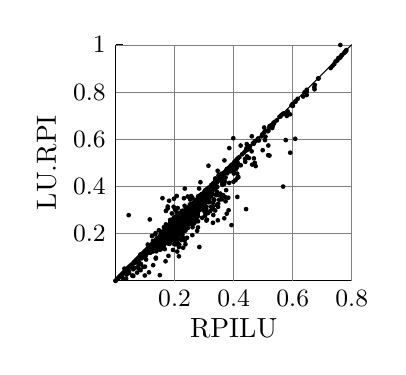
\begin{tikzpicture}

\draw (0,0) -- (3,0);
\node at (1.5,-0.6) {RPILU};
\node [anchor=north] at (0.75,0) {\small 0.2};
\draw (0.75,0) -- (0.75,0.1);
\draw [style=help lines] (0.75,0) -- (0.75,3);
\node [anchor=north] at (1.5,0) {\small 0.4};
\draw (1.5,0) -- (1.5,0.1);
\draw [style=help lines] (1.5,0) -- (1.5,3);
\node [anchor=north] at (2.25,0) {\small 0.6};
\draw (2.25,0) -- (2.25,0.1);
\draw [style=help lines] (2.25,0) -- (2.25,3);
\node [anchor=north] at (3,0) {\small 0.8};
\draw (3,0) -- (3,0.1);
\draw [style=help lines] (3,0) -- (3,3);
\draw (0,0) -- (0,3);
\node [rotate=90] at (-2.5em,1.5) {LU.RPI};
\node [anchor=east] at (0,0.599) {\small 0.2};
\draw (0,0.599) -- (0.1,0.599);
\draw [style=help lines] (0,0.599) -- (3,0.599);
\node [anchor=east] at (0,1.198) {\small 0.4};
\draw (0,1.198) -- (0.1,1.198);
\draw [style=help lines] (0,1.198) -- (3,1.198);
\node [anchor=east] at (0,1.797) {\small 0.6};
\draw (0,1.797) -- (0.1,1.797);
\draw [style=help lines] (0,1.797) -- (3,1.797);
\node [anchor=east] at (0,2.396) {\small 0.8};
\draw (0,2.396) -- (0.1,2.396);
\draw [style=help lines] (0,2.396) -- (3,2.396);
\node [anchor=east] at (0,2.995) {\small 1};
\draw (0,2.995) -- (0.1,2.995);
\draw [style=help lines] (0,2.995) -- (3,2.995);
\foreach \pos in {
	(0.000000, 0.000000),
	(0.022556, 0.022556),
	(0.028846, 0.028846),
	(0.034575, 0.033771),
	(0.039735, 0.039735),
	(0.047782, 0.047782),
	(0.055046, 0.055046),
	(0.060000, 0.060000),
	(0.065534, 0.065534),
	(0.089300, 0.036203),
	(0.072680, 0.069938),
	(0.075949, 0.075949),
	(0.083333, 0.083333),
	(0.090106, 0.084806),
	(0.092593, 0.092593),
	(0.134328, 0.026866),
	(0.099919, 0.099919),
	(0.104966, 0.104966),
	(0.110092, 0.110092),
	(0.114504, 0.114504),
	(0.142105, 0.078947),
	(0.122041, 0.122041),
	(0.128571, 0.128571),
	(0.113402, 0.154639),
	(0.136364, 0.136364),
	(0.172727, 0.100000),
	(0.142012, 0.142012),
	(0.149701, 0.141340),
	(0.169014, 0.118310),
	(0.146341, 0.146341),
	(0.156632, 0.139699),
	(0.147337, 0.152663),
	(0.155592, 0.150729),
	(0.156780, 0.156780),
	(0.213198, 0.065990),
	(0.218182, 0.062338),
	(0.162712, 0.162712),
	(0.225606, 0.061529),
	(0.168000, 0.168000),
	(0.173077, 0.173077),
	(0.183406, 0.170306),
	(0.177515, 0.177515),
	(0.182657, 0.182657),
	(0.224525, 0.145941),
	(0.190909, 0.190909),
	(0.195918, 0.195918),
	(0.204545, 0.204545),
	(0.273399, 0.103448),
	(0.244616, 0.163705),
	(0.214395, 0.211973),
	(0.223520, 0.221051),
	(0.233272, 0.225348),
	(0.233010, 0.233010),
	(0.292018, 0.157629),
	(0.239276, 0.238786),
	(0.287671, 0.179795),
	(0.245617, 0.240625),
	(0.255783, 0.231502),
	(0.318408, 0.134328),
	(0.248902, 0.248262),
	(0.256984, 0.242163),
	(0.266199, 0.239652),
	(0.257818, 0.250306),
	(0.256243, 0.256243),
	(0.293392, 0.222026),
	(0.262173, 0.258950),
	(0.270626, 0.252074),
	(0.265161, 0.264328),
	(0.285714, 0.244898),
	(0.273191, 0.259315),
	(0.371429, 0.066667),
	(0.271577, 0.265890),
	(0.295549, 0.239130),
	(0.276230, 0.270002),
	(0.321429, 0.214286),
	(0.282602, 0.268906),
	(0.276923, 0.276923),
	(0.352941, 0.176471),
	(0.283837, 0.278990),
	(0.287296, 0.286393),
	(0.292768, 0.289577),
	(0.374026, 0.179221),
	(0.298169, 0.292570),
	(0.306519, 0.285177),
	(0.298913, 0.298913),
	(0.304424, 0.302279),
	(0.309164, 0.307058),
	(0.331579, 0.284211),
	(0.424779, 0.106195),
	(0.320269, 0.300061),
	(0.317048, 0.308147),
	(0.325513, 0.303349),
	(0.316034, 0.315732),
	(0.321753, 0.312753),
	(0.328846, 0.313074),
	(0.321429, 0.321429),
	(0.315600, 0.333600),
	(0.327681, 0.321887),
	(0.328222, 0.327992),
	(0.339523, 0.318974),
	(0.333836, 0.325813),
	(0.332547, 0.332547),
	(0.387818, 0.269074),
	(0.346696, 0.324825),
	(0.339851, 0.332933),
	(0.365596, 0.305505),
	(0.339223, 0.339223),
	(0.345858, 0.338623),
	(0.354665, 0.329943),
	(0.350597, 0.334427),
	(0.344828, 0.344828),
	(0.372407, 0.323462),
	(0.358391, 0.339402),
	(0.353547, 0.345350),
	(0.380669, 0.315469),
	(0.351792, 0.351792),
	(0.371501, 0.333585),
	(0.358804, 0.348837),
	(0.367848, 0.341294),
	(0.357869, 0.356265),
	(0.364317, 0.351295),
	(0.387746, 0.329980),
	(0.371588, 0.350450),
	(0.364911, 0.357650),
	(0.381379, 0.345599),
	(0.364331, 0.363747),
	(0.478022, 0.197802),
	(0.373575, 0.359966),
	(0.369200, 0.367466),
	(0.382118, 0.361166),
	(0.377281, 0.366754),
	(0.372912, 0.372716),
	(0.388171, 0.356834),
	(0.382585, 0.369812),
	(0.388285, 0.364115),
	(0.378198, 0.377152),
	(0.398700, 0.357278),
	(0.384296, 0.377453),
	(0.393204, 0.369434),
	(0.407384, 0.356271),
	(0.385553, 0.383470),
	(0.393284, 0.376153),
	(0.401035, 0.372918),
	(0.396015, 0.381505),
	(0.389938, 0.388263),
	(0.413198, 0.368546),
	(0.396067, 0.389045),
	(0.402991, 0.387432),
	(0.396042, 0.395185),
	(0.402941, 0.395548),
	(0.408411, 0.390075),
	(0.419197, 0.380041),
	(0.441445, 0.355440),
	(0.562500, 0.071303),
	(0.415160, 0.388031),
	(0.403036, 0.402334),
	(0.413967, 0.396328),
	(0.419955, 0.392822),
	(0.411514, 0.402210),
	(0.447395, 0.364600),
	(0.408649, 0.408649),
	(0.445109, 0.371866),
	(0.415245, 0.407420),
	(0.422217, 0.400362),
	(0.510550, 0.282110),
	(0.427615, 0.397389),
	(0.414543, 0.413556),
	(0.420526, 0.412846),
	(0.512195, 0.292683),
	(0.426119, 0.408356),
	(0.435575, 0.401910),
	(0.420382, 0.420382),
	(0.431756, 0.413854),
	(0.425119, 0.424109),
	(0.432035, 0.420493),
	(0.450180, 0.401438),
	(0.477465, 0.372692),
	(0.461794, 0.392027),
	(0.428994, 0.428823),
	(0.438054, 0.421340),
	(0.436027, 0.429220),
	(0.409938, 0.459627),
	(0.447597, 0.423215),
	(0.436341, 0.435256),
	(0.460086, 0.411863),
	(0.443121, 0.432916),
	(0.452293, 0.427054),
	(0.442095, 0.439511),
	(0.449406, 0.432958),
	(0.484552, 0.397732),
	(0.469972, 0.415609),
	(0.450353, 0.439107),
	(0.463486, 0.425322),
	(0.445398, 0.445398),
	(0.458161, 0.434802),
	(0.485346, 0.411489),
	(0.450000, 0.450000),
	(0.474719, 0.424382),
	(0.455722, 0.445064),
	(0.518575, 0.373010),
	(0.455963, 0.451241),
	(0.510067, 0.389262),
	(0.473684, 0.435512),
	(0.464104, 0.448813),
	(0.457530, 0.457061),
	(0.469978, 0.447477),
	(0.464516, 0.454888),
	(0.478528, 0.441718),
	(0.486281, 0.436796),
	(0.462555, 0.462555),
	(0.472448, 0.453274),
	(0.468771, 0.459315),
	(0.501044, 0.426309),
	(0.467207, 0.466364),
	(0.479418, 0.454185),
	(0.508541, 0.421813),
	(0.486128, 0.449186),
	(0.478095, 0.460501),
	(0.473340, 0.468009),
	(0.484629, 0.459797),
	(0.474194, 0.474194),
	(0.503753, 0.443668),
	(0.483933, 0.466451),
	(0.482248, 0.473595),
	(0.498943, 0.458019),
	(0.479079, 0.478819),
	(0.491125, 0.466543),
	(0.489833, 0.472916),
	(0.505265, 0.456647),
	(0.635294, 0.247059),
	(0.484024, 0.482688),
	(0.496066, 0.470357),
	(0.490206, 0.480833),
	(0.514779, 0.455160),
	(0.564838, 0.393516),
	(0.510811, 0.462162),
	(0.488566, 0.488107),
	(0.497297, 0.481081),
	(0.474820, 0.505290),
	(0.545670, 0.427943),
	(0.508184, 0.473434),
	(0.488141, 0.494578),
	(0.496286, 0.487196),
	(0.503059, 0.485419),
	(0.495438, 0.493728),
	(0.512725, 0.477815),
	(0.510071, 0.483938),
	(0.503035, 0.491646),
	(0.499016, 0.499016),
	(0.523617, 0.473310),
	(0.518080, 0.483068),
	(0.506829, 0.497856),
	(0.582329, 0.407631),
	(0.513793, 0.493103),
	(0.504498, 0.504355),
	(0.539825, 0.467488),
	(0.520134, 0.491691),
	(0.516993, 0.498564),
	(0.510444, 0.505949),
	(0.565949, 0.443248),
	(0.528275, 0.492559),
	(0.523609, 0.499449),
	(0.516563, 0.507589),
	(0.592405, 0.417722),
	(0.513389, 0.513284),
	(0.523618, 0.505588),
	(0.546039, 0.481799),
	(0.579512, 0.441951),
	(0.522155, 0.511461),
	(0.531335, 0.502141),
	(0.462295, 0.567213),
	(0.518894, 0.516913),
	(0.529104, 0.508479),
	(0.538988, 0.498778),
	(0.515702, 0.525620),
	(0.525646, 0.517133),
	(0.556681, 0.483823),
	(0.523223, 0.522746),
	(0.549745, 0.496173),
	(0.543825, 0.505670),
	(0.672091, 0.315881),
	(0.539137, 0.511312),
	(0.625418, 0.401709),
	(0.531310, 0.521010),
	(0.577982, 0.469266),
	(0.528235, 0.526466),
	(0.559050, 0.497695),
	(0.538117, 0.521818),
	(0.607880, 0.439024),
	(0.534552, 0.527315),
	(0.545687, 0.515882),
	(0.556385, 0.510104),
	(0.583287, 0.479666),
	(0.534247, 0.534247),
	(0.548682, 0.522862),
	(0.540110, 0.532203),
	(0.575860, 0.498788),
	(0.538043, 0.540583),
	(0.615471, 0.450673),
	(0.550128, 0.529679),
	(0.556675, 0.525795),
	(0.544432, 0.541934),
	(0.549581, 0.538480),
	(0.570624, 0.517061),
	(0.502392, 0.588517),
	(0.547297, 0.547297),
	(0.564342, 0.530161),
	(0.557851, 0.537190),
	(0.554382, 0.543358),
	(0.579525, 0.518991),
	(0.553126, 0.549707),
	(0.560810, 0.546724),
	(0.567796, 0.540317),
	(0.574570, 0.533723),
	(0.586726, 0.520354),
	(0.557763, 0.555501),
	(0.568089, 0.547049),
	(0.508619, 0.604654),
	(0.579177, 0.540221),
	(0.564800, 0.557593),
	(0.573043, 0.550684),
	(0.582176, 0.545902),
	(0.564516, 0.564516),
	(0.614787, 0.509510),
	(0.574274, 0.557056),
	(0.588620, 0.543857),
	(0.571084, 0.563855),
	(0.626620, 0.504122),
	(0.584448, 0.556856),
	(0.571217, 0.570848),
	(0.579678, 0.564971),
	(0.649264, 0.484605),
	(0.596143, 0.548802),
	(0.619091, 0.523636),
	(0.625467, 0.518506),
	(0.659864, 0.476190),
	(0.595420, 0.556161),
	(0.604964, 0.546019),
	(0.576528, 0.576191),
	(0.582152, 0.573095),
	(0.606843, 0.552821),
	(0.613559, 0.545502),
	(0.593662, 0.567306),
	(0.582296, 0.580963),
	(0.589167, 0.574444),
	(0.600292, 0.563822),
	(0.627629, 0.535851),
	(0.606382, 0.561896),
	(0.611448, 0.556808),
	(0.596774, 0.572581),
	(0.588198, 0.582487),
	(0.642857, 0.522321),
	(0.730128, 0.391560),
	(0.621888, 0.548929),
	(0.594298, 0.580238),
	(0.686551, 0.468547),
	(0.607078, 0.568398),
	(0.589037, 0.588882),
	(0.604436, 0.576630),
	(0.617414, 0.564644),
	(0.648491, 0.529698),
	(0.613145, 0.570312),
	(0.577154, 0.607132),
	(0.596933, 0.588314),
	(0.602496, 0.585477),
	(0.612189, 0.577036),
	(0.641385, 0.546938),
	(0.584714, 0.607717),
	(0.597716, 0.595178),
	(0.618118, 0.573994),
	(0.631521, 0.559933),
	(0.550435, 0.641739),
	(0.609499, 0.587071),
	(0.604396, 0.593407),
	(0.166667, 0.833333),
	(0.656665, 0.540089),
	(0.632453, 0.568569),
	(0.602564, 0.600586),
	(0.618432, 0.584552),
	(0.615015, 0.589980),
	(0.612527, 0.595695),
	(0.633271, 0.574624),
	(0.609795, 0.601152),
	(0.646532, 0.562068),
	(0.606099, 0.606099),
	(0.626006, 0.586296),
	(0.619847, 0.594326),
	(0.591671, 0.623771),
	(0.641534, 0.573620),
	(0.645626, 0.569214),
	(0.804598, 0.310345),
	(0.613135, 0.606539),
	(0.608932, 0.612200),
	(0.618696, 0.602895),
	(0.638037, 0.582822),
	(0.657568, 0.563275),
	(0.628429, 0.596010),
	(0.633910, 0.590614),
	(0.672800, 0.545997),
	(0.783708, 0.370787),
	(0.665525, 0.555694),
	(0.651270, 0.573326),
	(0.692557, 0.524272),
	(0.616214, 0.612619),
	(0.645117, 0.584594),
	(0.627026, 0.603992),
	(0.666000, 0.564000),
	(0.709139, 0.508787),
	(0.624464, 0.609979),
	(0.642222, 0.593072),
	(0.623385, 0.617113),
	(0.635533, 0.604928),
	(0.687943, 0.546099),
	(0.745701, 0.464343),
	(0.667263, 0.573345),
	(0.615142, 0.629338),
	(0.631473, 0.614063),
	(0.654640, 0.589699),
	(0.623403, 0.623311),
	(0.661538, 0.582692),
	(0.629281, 0.621349),
	(0.646078, 0.604077),
	(0.707460, 0.533173),
	(0.652958, 0.601164),
	(0.643712, 0.611448),
	(0.636092, 0.620371),
	(0.628530, 0.628292),
	(0.664550, 0.591534),
	(0.435311, 0.778413),
	(0.654019, 0.609176),
	(0.636640, 0.627849),
	(0.650231, 0.615342),
	(0.665272, 0.600000),
	(0.642803, 0.624218),
	(0.767666, 0.462527),
	(0.634691, 0.633976),
	(0.641523, 0.631844),
	(0.651037, 0.622877),
	(0.656997, 0.617747),
	(0.675000, 0.600000),
	(0.639431, 0.638471),
	(0.722672, 0.542510),
	(0.679455, 0.595916),
	(0.693632, 0.580034),
	(0.649851, 0.628846),
	(0.665706, 0.612366),
	(0.645451, 0.637444),
	(0.658537, 0.625492),
	(0.756164, 0.507763),
	(0.684898, 0.600816),
	(0.657046, 0.631579),
	(0.652854, 0.636264),
	(0.805132, 0.428571),
	(0.646637, 0.643330),
	(0.714599, 0.566959),
	(0.681655, 0.607914),
	(0.697674, 0.594226),
	(0.614597, 0.679898),
	(0.666932, 0.628685),
	(0.659762, 0.637481),
	(0.654601, 0.643033),
	(0.650239, 0.649197),
	(0.632342, 0.668030),
	(0.627804, 0.674778),
	(0.690275, 0.611009),
	(0.675870, 0.627167),
	(0.659734, 0.646423),
	(0.670227, 0.636764),
	(0.655918, 0.651820),
	(0.699847, 0.604580),
	(0.645228, 0.663555),
	(0.783251, 0.497537),
	(0.685345, 0.626232),
	(0.661905, 0.652381),
	(0.750228, 0.548558),
	(0.666956, 0.647416),
	(0.679142, 0.634642),
	(0.702083, 0.610417),
	(0.657919, 0.657919),
	(0.809524, 0.460317),
	(0.672229, 0.644492),
	(0.708753, 0.604142),
	(0.678296, 0.644823),
	(0.663634, 0.660104),
	(0.668267, 0.655541),
	(0.690801, 0.632027),
	(0.673912, 0.653249),
	(0.733645, 0.586449),
	(0.645472, 0.685934),
	(0.709167, 0.620000),
	(0.667817, 0.664821),
	(0.653303, 0.680638),
	(0.704545, 0.627990),
	(0.688243, 0.646099),
	(0.681946, 0.652947),
	(0.674586, 0.660585),
	(0.759598, 0.560786),
	(0.695131, 0.641948),
	(0.727695, 0.605948),
	(0.715607, 0.622199),
	(0.672750, 0.670723),
	(0.681770, 0.661947),
	(0.714153, 0.628272),
	(0.695445, 0.649706),
	(0.701768, 0.643099),
	(0.692106, 0.655368),
	(0.681381, 0.668565),
	(0.858871, 0.419355),
	(0.677905, 0.675292),
	(0.691437, 0.661702),
	(0.798065, 0.529625),
	(0.755011, 0.593318),
	(0.639756, 0.716299),
	(0.685007, 0.674421),
	(0.740389, 0.613890),
	(0.702323, 0.658023),
	(0.760956, 0.589641),
	(0.697838, 0.663454),
	(0.691631, 0.670355),
	(0.719727, 0.642096),
	(0.725847, 0.635593),
	(0.684625, 0.680847),
	(0.778462, 0.575385),
	(0.698014, 0.670765),
	(0.703753, 0.665604),
	(0.718674, 0.651363),
	(0.694691, 0.677396),
	(0.710866, 0.660603),
	(0.686636, 0.686636),
	(0.737750, 0.634301),
	(0.693195, 0.683371),
	(0.730858, 0.643852),
	(0.745050, 0.628713),
	(0.700921, 0.677735),
	(0.717000, 0.663000),
	(0.712093, 0.668372),
	(0.707565, 0.673236),
	(0.692255, 0.689973),
	(0.727506, 0.653114),
	(0.787836, 0.579987),
	(0.701814, 0.684113),
	(0.755046, 0.628440),
	(0.700204, 0.690245),
	(0.764940, 0.619124),
	(0.837669, 0.516673),
	(0.715048, 0.676381),
	(0.720372, 0.670711),
	(0.725260, 0.666290),
	(0.734003, 0.656683),
	(0.709901, 0.684158),
	(0.691031, 0.703477),
	(0.749473, 0.641260),
	(0.698207, 0.696795),
	(0.707204, 0.690178),
	(0.716269, 0.682765),
	(0.721120, 0.679113),
	(0.737810, 0.662641),
	(0.703761, 0.699454),
	(0.753434, 0.646501),
	(0.730435, 0.672671),
	(0.713488, 0.691141),
	(0.768029, 0.632212),
	(0.710507, 0.696754),
	(0.725543, 0.684783),
	(0.720139, 0.691148),
	(0.780892, 0.622140),
	(0.689826, 0.722395),
	(0.706656, 0.706080),
	(0.743286, 0.667491),
	(0.716995, 0.697109),
	(0.799166, 0.602503),
	(0.713555, 0.702659),
	(0.888185, 0.463520),
	(0.753846, 0.661538),
	(0.739053, 0.678284),
	(0.760112, 0.655558),
	(0.723550, 0.697002),
	(0.729192, 0.691534),
	(0.719814, 0.703722),
	(0.712941, 0.711195),
	(0.781395, 0.637209),
	(0.749400, 0.677342),
	(0.743325, 0.684644),
	(0.719879, 0.709754),
	(0.727979, 0.701947),
	(0.736602, 0.693350),
	(0.837523, 0.569992),
	(0.717621, 0.715998),
	(0.805049, 0.617111),
	(0.775382, 0.654944),
	(0.877917, 0.510245),
	(0.835025, 0.577845),
	(0.745261, 0.690470),
	(0.754330, 0.680868),
	(0.736248, 0.701551),
	(0.759462, 0.677040),
	(0.723649, 0.716047),
	(0.728155, 0.711564),
	(0.772542, 0.663451),
	(0.862479, 0.541907),
	(0.844833, 0.569826),
	(0.752554, 0.688536),
	(0.695438, 0.747226),
	(0.723094, 0.723094),
	(0.748297, 0.697200),
	(0.743297, 0.703035),
	(0.765550, 0.679426),
	(0.739401, 0.708395),
	(0.728958, 0.719328),
	(0.711588, 0.736556),
	(0.734543, 0.714598),
	(0.773797, 0.672467),
	(0.762513, 0.687611),
	(0.729273, 0.725609),
	(0.758709, 0.695370),
	(0.737315, 0.720115),
	(0.794891, 0.656500),
	(0.786157, 0.667333),
	(0.757036, 0.702178),
	(0.749600, 0.711159),
	(0.832646, 0.612552),
	(0.743611, 0.718056),
	(0.849903, 0.589286),
	(0.736728, 0.726701),
	(0.772306, 0.689420),
	(0.794444, 0.663889),
	(0.767427, 0.695481),
	(0.763417, 0.700719),
	(0.693407, 0.772294),
	(0.787390, 0.676320),
	(0.756026, 0.711261),
	(0.780930, 0.684791),
	(0.736581, 0.732715),
	(0.749433, 0.719929),
	(0.745903, 0.724891),
	(0.770992, 0.700382),
	(0.756898, 0.718839),
	(0.743192, 0.734115),
	(0.762400, 0.714218),
	(0.776899, 0.698576),
	(0.804787, 0.667355),
	(0.749308, 0.730391),
	(0.773606, 0.706485),
	(0.741922, 0.740529),
	(0.758034, 0.727914),
	(0.788860, 0.694498),
	(0.772023, 0.714556),
	(0.765598, 0.721556),
	(0.750887, 0.740307),
	(0.801902, 0.684899),
	(0.820836, 0.662851),
	(0.833818, 0.648719),
	(0.747540, 0.746884),
	(0.764562, 0.729843),
	(0.717493, 0.776240),
	(0.757756, 0.737439),
	(0.808853, 0.682093),
	(0.770543, 0.725870),
	(0.908016, 0.545735),
	(0.755459, 0.745477),
	(0.784788, 0.714745),
	(0.780686, 0.719450),
	(0.749642, 0.752504),
	(0.763397, 0.739607),
	(0.804878, 0.695122),
	(0.798344, 0.704357),
	(0.778997, 0.727334),
	(0.793072, 0.712220),
	(0.762316, 0.745895),
	(0.774810, 0.733654),
	(0.755824, 0.754010),
	(0.791336, 0.719819),
	(0.769400, 0.743808),
	(0.801639, 0.710656),
	(0.825460, 0.684952),
	(0.785349, 0.730919),
	(0.776047, 0.740931),
	(0.844161, 0.662409),
	(0.766390, 0.751600),
	(0.833583, 0.677005),
	(0.867151, 0.633627),
	(0.761000, 0.758549),
	(0.801223, 0.716727),
	(0.825656, 0.690962),
	(0.775531, 0.747757),
	(0.810154, 0.712769),
	(0.767986, 0.759034),
	(0.763838, 0.763838),
	(0.798184, 0.729050),
	(0.785145, 0.743410),
	(0.853571, 0.665476),
	(0.792930, 0.737185),
	(0.808355, 0.721301),
	(0.775504, 0.756545),
	(0.771622, 0.763888),
	(0.791440, 0.744015),
	(0.834646, 0.695283),
	(0.818913, 0.716692),
	(0.780504, 0.760343),
	(0.785739, 0.755478),
	(0.772714, 0.770354),
	(0.777710, 0.765752),
	(0.829037, 0.710153),
	(0.795670, 0.748309),
	(0.800772, 0.743526),
	(0.888205, 0.636665),
	(0.791700, 0.753769),
	(0.640449, 0.886838),
	(0.814012, 0.731443),
	(0.742650, 0.804719),
	(0.748385, 0.800054),
	(0.870377, 0.666786),
	(0.780034, 0.771681),
	(0.826341, 0.722079),
	(0.789068, 0.762774),
	(0.805343, 0.748215),
	(0.813369, 0.739572),
	(0.797379, 0.757213),
	(0.852420, 0.695017),
	(0.860104, 0.685665),
	(0.787865, 0.770228),
	(0.780508, 0.779549),
	(0.785828, 0.776315),
	(0.796694, 0.766092),
	(0.852273, 0.703877),
	(0.840864, 0.719057),
	(0.812561, 0.751717),
	(0.766616, 0.798701),
	(0.804159, 0.761059),
	(0.884116, 0.666833),
	(0.848532, 0.711746),
	(0.792832, 0.773823),
	(0.758146, 0.809196),
	(0.820798, 0.745584),
	(0.787294, 0.782469),
	(0.811512, 0.759594),
	(0.799408, 0.772761),
	(0.806281, 0.768352),
	(0.715026, 0.854922),
	(0.845329, 0.726901),
	(0.793786, 0.783590),
	(0.783590, 0.795414),
	(0.852905, 0.720643),
	(0.790927, 0.790213),
	(0.812322, 0.768246),
	(0.892324, 0.673901),
	(0.834194, 0.745161),
	(0.800259, 0.781806),
	(0.820212, 0.763900),
	(0.797411, 0.788390),
	(0.810319, 0.775799),
	(0.842178, 0.743195),
	(0.885005, 0.692503),
	(0.807352, 0.783191),
	(0.834846, 0.754133),
	(0.796970, 0.795455),
	(0.831463, 0.760320),
	(0.882779, 0.701964),
	(0.902846, 0.676281),
	(0.803737, 0.792074),
	(0.825267, 0.771823),
	(0.830919, 0.767571),
	(0.662148, 0.917570),
	(0.811606, 0.789746),
	(0.819060, 0.782743),
	(0.850427, 0.749288),
	(0.805046, 0.798165),
	(0.975494, 0.579371),
	(0.904252, 0.685448),
	(0.898413, 0.693477),
	(0.829018, 0.776724),
	(0.863702, 0.738038),
	(0.843613, 0.761496),
	(0.836738, 0.769905),
	(0.918159, 0.670784),
	(0.811740, 0.796925),
	(0.820085, 0.788967),
	(0.784393, 0.824618),
	(0.826874, 0.783488),
	(0.884649, 0.718127),
	(0.872278, 0.733413),
	(0.810342, 0.803291),
	(0.817737, 0.796142),
	(0.845136, 0.768365),
	(0.835543, 0.781992),
	(0.840160, 0.777358),
	(0.828167, 0.790971),
	(0.859098, 0.760264),
	(0.822704, 0.799745),
	(1.064516, 0.429007),
	(0.819021, 0.805171),
	(0.868207, 0.752446),
	(0.815343, 0.810193),
	(0.882192, 0.736986),
	(0.856416, 0.766905),
	(0.839115, 0.788036),
	(0.832525, 0.795241),
	(0.662136, 0.942718),
	(0.850365, 0.777372),
	(0.813869, 0.817518),
	(0.876133, 0.752394),
	(0.900196, 0.724341),
	(0.826203, 0.807801),
	(0.861770, 0.770946),
	(0.833288, 0.802029),
	(0.848035, 0.786442),
	(0.857408, 0.777055),
	(0.887976, 0.742698),
	(0.841775, 0.794711),
	(0.823852, 0.815434),
	(0.876486, 0.762641),
	(0.904517, 0.729794),
	(0.840140, 0.803307),
	(0.871394, 0.770357),
	(0.780466, 0.862375),
	(0.846894, 0.797900),
	(0.853178, 0.791633),
	(0.836333, 0.809603),
	(0.831954, 0.814131),
	(0.860825, 0.784149),
	(0.828008, 0.820489),
	(0.870836, 0.776921),
	(0.827181, 0.826828),
	(0.786822, 0.865559),
	(0.838821, 0.816291),
	(0.849943, 0.805651),
	(0.864364, 0.790482),
	(0.855889, 0.799927),
	(0.799062, 0.857504),
	(0.845339, 0.811970),
	(0.835186, 0.823414),
	(0.874076, 0.784532),
	(0.893392, 0.762748),
	(0.887238, 0.770155),
	(0.927492, 0.722054),
	(0.756027, 0.900675),
	(0.833242, 0.829962),
	(0.910644, 0.744634),
	(0.933714, 0.717464),
	(0.841429, 0.825258),
	(0.850961, 0.816318),
	(0.861882, 0.806014),
	(0.873220, 0.795068),
	(0.884826, 0.782450),
	(0.895844, 0.770171),
	(0.835900, 0.835389),
	(0.869737, 0.800789),
	(0.848171, 0.825052),
	(0.841364, 0.832350),
	(0.917439, 0.749789),
	(0.856419, 0.819079),
	(0.938965, 0.723633),
	(0.868609, 0.809495),
	(0.913435, 0.758602),
	(0.877336, 0.801527),
	(0.847137, 0.834630),
	(0.900790, 0.776916),
	(0.895793, 0.782983),
	(0.855820, 0.826720),
	(0.888262, 0.792307),
	(0.844152, 0.840198),
	(0.884234, 0.797967),
	(0.861367, 0.822662),
	(0.978372, 0.679567),
	(0.866865, 0.819450),
	(0.877545, 0.809672),
	(0.737786, 0.939538),
	(0.923239, 0.758952),
	(0.857530, 0.833333),
	(0.946985, 0.730271),
	(0.862777, 0.828972),
	(0.846211, 0.846211),
	(0.890313, 0.800099),
	(0.884812, 0.808872),
	(0.877924, 0.818543),
	(0.852547, 0.846113),
	(0.859562, 0.839931),
	(0.933149, 0.759116),
	(0.871476, 0.831161),
	(0.902745, 0.797526),
	(0.878661, 0.824760),
	(0.897534, 0.805373),
	(0.939130, 0.756522),
	(0.851999, 0.853718),
	(0.596084, 1.048586),
	(0.868540, 0.837015),
	(0.859944, 0.847339),
	(0.876719, 0.834725),
	(0.885942, 0.826198),
	(0.857411, 0.857411),
	(0.838347, 0.876627),
	(0.867544, 0.848767),
	(0.952047, 0.753233),
	(0.894031, 0.821842),
	(1.036045, 0.634398),
	(0.900066, 0.816016),
	(0.978592, 0.720371),
	(0.790432, 0.923242),
	(0.905539, 0.811079),
	(0.874674, 0.844291),
	(0.884301, 0.834747),
	(0.863961, 0.856006),
	(0.926320, 0.790733),
	(0.953057, 0.759825),
	(0.920292, 0.800730),
	(0.896487, 0.827635),
	(0.874379, 0.852781),
	(0.977609, 0.732907),
	(0.865807, 0.862341),
	(0.881536, 0.847277),
	(0.893734, 0.834667),
	(0.680372, 1.016292),
	(0.902839, 0.825320),
	(0.969112, 0.749035),
	(0.957541, 0.765527),
	(0.845300, 0.887913),
	(0.954003, 0.770880),
	(0.917160, 0.814416),
	(0.976336, 0.742748),
	(0.894050, 0.841541),
	(0.871533, 0.864964),
	(0.888672, 0.847666),
	(0.881621, 0.855366),
	(0.906646, 0.830696),
	(0.878525, 0.861664),
	(0.993660, 0.726354),
	(0.926561, 0.811256),
	(0.870968, 0.870968),
	(0.895490, 0.848735),
	(0.890332, 0.854185),
	(0.900056, 0.843976),
	(0.878094, 0.867662),
	(0.919056, 0.826087),
	(0.935025, 0.808412),
	(0.941417, 0.800960),
	(0.925102, 0.822586),
	(0.887139, 0.863955),
	(0.876246, 0.876246),
	(0.917293, 0.833584),
	(0.892761, 0.860015),
	(0.907006, 0.846065),
	(0.882837, 0.871764),
	(0.865290, 0.890433),
	(0.903223, 0.852615),
	(0.900906, 0.860642),
	(0.892463, 0.869537),
	(0.880842, 0.881400),
	(1.003944, 0.738592),
	(0.930990, 0.828671),
	(1.046829, 0.677199),
	(0.911830, 0.853345),
	(0.887869, 0.879816),
	(0.909147, 0.859507),
	(0.940624, 0.825727),
	(0.895177, 0.875572),
	(0.945968, 0.822111),
	(0.888781, 0.886070),
	(0.940916, 0.832595),
	(0.954130, 0.818043),
	(0.907524, 0.869647),
	(0.895883, 0.881685),
	(0.901624, 0.876313),
	(0.886403, 0.892822),
	(0.923289, 0.855440),
	(0.984356, 0.785941),
	(0.933841, 0.846510),
	(0.894330, 0.888577),
	(0.915789, 0.866609),
	(0.953039, 0.826817),
	(0.909774, 0.875665),
	(0.902232, 0.885492),
	(0.907237, 0.881538),
	(1.002201, 0.772702),
	(0.942213, 0.845540),
	(0.925270, 0.864307),
	(0.919030, 0.872615),
	(0.953089, 0.835474),
	(0.916018, 0.878049),
	(0.939105, 0.853391),
	(0.902511, 0.892910),
	(1.016660, 0.760829),
	(0.936498, 0.860708),
	(0.899851, 0.899562),
	(0.910714, 0.888685),
	(0.931106, 0.868099),
	(0.919658, 0.882934),
	(0.961394, 0.837376),
	(0.972012, 0.825176),
	(0.908609, 0.895837),
	(0.937226, 0.867640),
	(0.741940, 1.041899),
	(0.934904, 0.873278),
	(0.902603, 0.907174),
	(0.967930, 0.837828),
	(0.927173, 0.882978),
	(0.963855, 0.843373),
	(0.990472, 0.814205),
	(0.934099, 0.879275),
	(0.915227, 0.899403),
	(0.920321, 0.894570),
	(0.959446, 0.854105),
	(0.940073, 0.876944),
	(0.910501, 0.907842),
	(0.988740, 0.822434),
	(0.954441, 0.862090),
	(1.033137, 0.766491),
	(0.983854, 0.830769),
	(0.936865, 0.886411),
	(0.922006, 0.903064),
	(0.917024, 0.908441),
	(1.048043, 0.754720),
	(0.955597, 0.869362),
	(0.929833, 0.898568),
	(0.978206, 0.846605),
	(0.877078, 0.951886),
	(0.964264, 0.863738),
	(0.970683, 0.857028),
	(0.917621, 0.914735),
	(0.947258, 0.884470),
	(1.020580, 0.798877),
	(0.936487, 0.898142),
	(0.926664, 0.908426),
	(0.933074, 0.903860),
	(0.958144, 0.877278),
	(0.953567, 0.882597),
	(0.923936, 0.915682),
	(0.943046, 0.896050),
	(1.026941, 0.800135),
	(0.917419, 0.924282),
	(0.964126, 0.875882),
	(0.975962, 0.865385),
	(0.956144, 0.889942),
	(0.930515, 0.916852),
	(0.941130, 0.906898),
	(0.926438, 0.922024),
	(0.951846, 0.897705),
	(0.963876, 0.884828),
	(0.938190, 0.915011),
	(0.984796, 0.865155),
	(0.926317, 0.929044),
	(0.958437, 0.897022),
	(0.951913, 0.904362),
	(0.932773, 0.925898),
	(0.943434, 0.918182),
	(0.948614, 0.913379),
	(0.984297, 0.876621),
	(0.958213, 0.907781),
	(0.938804, 0.929511),
	(0.945182, 0.924197),
	(0.968578, 0.899764),
	(0.951421, 0.919340),
	(0.964819, 0.905430),
	(0.990554, 0.878439),
	(0.935866, 0.936800),
	(0.959970, 0.914240),
	(0.974864, 0.898831),
	(1.008476, 0.863116),
	(1.046367, 0.816955),
	(0.777090, 1.076367),
	(1.014689, 0.857364),
	(0.966144, 0.912559),
	(0.971435, 0.906975),
	(0.985150, 0.896766),
	(1.032721, 0.842135),
	(0.944246, 0.940823),
	(0.953880, 0.931552),
	(0.969191, 0.918696),
	(0.993947, 0.892032),
	(0.962963, 0.928636),
	(0.950818, 0.941620),
	(1.005230, 0.883622),
	(1.012946, 0.875087),
	(0.981891, 0.911232),
	(0.947368, 0.947368),
	(0.959497, 0.936704),
	(1.025650, 0.867351),
	(0.996527, 0.904242),
	(0.955972, 0.947215),
	(1.020066, 0.879971),
	(1.006866, 0.895696),
	(0.962930, 0.942902),
	(0.988004, 0.917946),
	(1.045652, 0.852545),
	(0.978406, 0.929970),
	(0.974616, 0.935026),
	(0.955121, 0.955121),
	(1.038866, 0.867135),
	(1.014085, 0.896543),
	(0.944867, 0.969540),
	(1.005386, 0.906643),
	(0.988318, 0.925234),
	(0.968382, 0.946445),
	(0.962523, 0.957038),
	(1.031729, 0.882709),
	(0.982259, 0.937653),
	(0.974725, 0.948023),
	(1.100248, 0.799505),
	(0.868849, 1.047563),
	(1.011078, 0.912584),
	(0.995803, 0.931275),
	(0.964286, 0.964286),
	(0.989897, 0.938886),
	(0.981510, 0.948772),
	(1.002850, 0.927117),
	(1.007210, 0.922713),
	(0.969974, 0.961845),
	(0.977804, 0.955010),
	(1.038236, 0.890168),
	(0.987082, 0.952056),
	(0.977367, 0.963062),
	(0.975960, 0.969894),
	(0.984964, 0.961314),
	(1.032286, 0.910995),
	(1.017190, 0.929587),
	(1.012690, 0.936548),
	(1.006697, 0.944932),
	(0.977625, 0.975877),
	(1.002909, 0.951174),
	(0.995401, 0.961165),
	(1.153727, 0.763975),
	(0.990729, 0.967985),
	(0.986849, 0.973752),
	(1.023445, 0.938756),
	(1.010350, 0.953835),
	(0.985651, 0.980049),
	(1.066826, 0.894988),
	(0.993649, 0.976063),
	(1.160890, 0.774444),
	(1.010157, 0.964705),
	(1.002429, 0.975106),
	(1.066248, 0.905206),
	(1.049847, 0.924212),
	(0.995857, 0.982361),
	(1.017134, 0.960726),
	(0.990847, 0.989220),
	(1.134735, 0.820612),
	(1.024414, 0.954816),
	(0.947906, 1.031003),
	(1.032319, 0.949144),
	(1.010360, 0.973492),
	(1.040856, 0.942857),
	(1.025228, 0.961834),
	(1.002887, 0.986009),
	(0.916307, 1.069543),
	(0.996631, 0.996301),
	(1.011309, 0.981826),
	(1.030220, 0.966117),
	(1.004433, 0.993411),
	(1.037749, 0.963624),
	(1.002710, 1.000087),
	(1.028948, 0.973249),
	(1.011217, 0.993018),
	(1.017250, 0.989691),
	(1.008712, 0.998823),
	(1.023223, 0.986995),
	(1.045581, 0.966648),
	(1.056832, 0.954348),
	(1.095050, 0.910922),
	(1.038595, 0.975044),
	(1.145148, 0.848035),
	(1.019690, 0.996062),
	(1.014603, 1.002336),
	(1.037290, 0.984238),
	(1.130740, 0.876276),
	(1.014960, 1.008472),
	(1.024666, 1.001007),
	(1.090523, 0.929279),
	(1.035659, 0.993698),
	(1.008896, 1.023075),
	(1.016542, 1.016323),
	(0.974684, 1.056962),
	(1.062660, 0.969437),
	(1.097439, 0.930401),
	(1.053140, 0.980676),
	(1.236818, 0.736355),
	(1.147715, 0.870351),
	(0.959367, 1.074934),
	(1.090365, 0.941893),
	(1.034849, 1.002953),
	(1.123512, 0.903026),
	(1.040462, 0.999277),
	(1.020870, 1.020870),
	(1.074184, 0.964615),
	(1.065608, 0.978354),
	(1.027167, 1.019470),
	(1.059521, 0.986210),
	(1.035159, 1.011883),
	(1.101762, 0.941806),
	(1.147132, 0.889027),
	(1.035623, 1.018609),
	(1.045283, 1.009434),
	(1.029166, 1.026086),
	(1.060339, 0.994546),
	(1.173711, 0.859021),
	(1.042226, 1.018042),
	(1.052583, 1.008303),
	(1.035938, 1.025951),
	(1.048247, 1.015409),
	(1.093884, 0.966887),
	(1.065789, 0.998120),
	(1.032811, 1.032395),
	(1.086336, 0.977702),
	(1.058786, 1.009126),
	(1.091734, 0.973790),
	(0.879934, 1.170301),
	(1.043603, 1.028920),
	(1.083896, 0.991470),
	(1.143168, 0.922700),
	(1.149697, 0.915758),
	(1.077892, 0.999707),
	(1.091364, 0.990734),
	(1.096560, 0.986317),
	(1.066794, 1.018766),
	(1.062950, 1.030576),
	(1.053286, 1.041741),
	(1.113034, 0.978042),
	(1.086230, 1.007869),
	(1.079200, 1.018635),
	(1.128039, 0.964301),
	(1.101259, 0.996390),
	(1.069052, 1.035786),
	(1.078813, 1.026612),
	(1.155328, 0.940425),
	(1.134454, 0.965839),
	(1.056362, 1.052946),
	(1.091105, 1.017271),
	(1.201560, 0.884265),
	(1.077397, 1.032982),
	(1.127451, 0.980392),
	(1.068397, 1.045973),
	(1.241476, 0.835138),
	(1.065393, 1.051795),
	(1.075812, 1.041717),
	(1.081860, 1.037140),
	(1.062668, 1.057278),
	(1.048622, 1.072665),
	(1.082350, 1.044638),
	(1.076031, 1.052506),
	(1.102555, 1.027109),
	(1.098513, 1.031599),
	(1.066941, 1.066281),
	(1.298528, 0.767694),
	(1.117200, 1.016177),
	(1.073264, 1.062951),
	(1.088855, 1.047266),
	(1.079204, 1.057965),
	(1.108909, 1.030550),
	(1.085311, 1.058414),
	(1.139928, 1.000241),
	(1.131139, 1.010487),
	(1.092143, 1.053088),
	(1.144879, 0.995957),
	(1.074146, 1.072314),
	(1.082523, 1.064447),
	(1.122555, 1.023993),
	(1.113313, 1.035110),
	(1.081730, 1.071618),
	(1.100501, 1.052916),
	(1.088582, 1.065647),
	(1.078443, 1.078128),
	(1.096237, 1.061157),
	(1.074480, 1.085980),
	(1.115066, 1.044799),
	(1.120908, 1.042504),
	(1.098383, 1.067385),
	(1.145827, 1.020624),
	(1.213831, 0.940183),
	(1.233313, 0.915780),
	(1.127034, 1.044207),
	(1.109126, 1.064854),
	(1.115439, 1.060264),
	(1.088946, 1.088946),
	(1.102851, 1.076435),
	(1.095591, 1.083879),
	(1.119672, 1.067016),
	(1.144638, 1.041102),
	(1.114053, 1.074661),
	(1.265415, 0.891947),
	(1.186272, 0.995693),
	(1.112153, 1.080953),
	(1.093664, 1.100043),
	(1.168521, 1.025437),
	(1.105612, 1.094898),
	(1.183099, 1.010834),
	(1.154525, 1.043822),
	(1.120280, 1.080944),
	(1.238444, 0.945290),
	(1.103798, 1.101846),
	(1.130999, 1.077498),
	(1.148479, 1.064255),
	(1.129749, 1.085552),
	(1.123034, 1.095771),
	(1.114072, 1.105408),
	(1.190251, 1.027759),
	(1.136292, 1.088748),
	(1.122930, 1.103362),
	(1.120709, 1.110714),
	(1.136653, 1.096723),
	(1.061292, 1.171171),
	(1.152476, 1.085593),
	(1.129691, 1.114044),
	(1.187964, 1.053302),
	(1.123624, 1.123430),
	(1.239249, 0.994852),
	(1.167707, 1.082813),
	(1.381020, 0.793201),
	(1.133134, 1.119113),
	(1.182573, 1.067105),
	(1.163695, 1.091113),
	(1.130036, 1.127464),
	(1.143927, 1.114086),
	(1.150342, 1.109923),
	(1.159054, 1.103589),
	(1.195920, 1.065738),
	(1.192339, 1.072488),
	(1.302281, 0.938459),
	(1.137069, 1.134446),
	(1.287447, 0.960531),
	(1.143766, 1.131043),
	(1.157691, 1.123402),
	(1.142905, 1.140169),
	(1.172671, 1.116432),
	(1.140000, 1.150000),
	(1.164706, 1.125642),
	(1.246615, 1.034910),
	(1.211951, 1.075587),
	(1.146550, 1.145773),
	(1.254972, 1.026084),
	(1.153028, 1.149660),
	(1.303531, 0.977221),
	(1.168260, 1.137667),
	(1.159404, 1.148963),
	(1.472189, 0.706509),
	(1.160781, 1.155669),
	(1.167316, 1.156308),
	(1.160959, 1.163894),
	(1.197578, 1.131847),
	(1.412117, 0.851515),
	(1.181159, 1.153623),
	(1.225136, 1.107131),
	(1.078030, 1.251429),
	(1.197446, 1.138978),
	(1.233697, 1.099884),
	(1.174062, 1.164968),
	(1.178065, 1.170501),
	(1.190635, 1.164103),
	(1.200268, 1.157989),
	(1.315578, 1.028300),
	(1.183424, 1.183148),
	(1.190342, 1.176379),
	(1.275787, 1.092220),
	(1.280041, 1.087576),
	(1.198622, 1.177956),
	(1.212305, 1.169464),
	(1.207103, 1.175533),
	(1.202442, 1.183953),
	(1.435841, 0.894933),
	(1.229266, 1.168602),
	(1.210157, 1.193154),
	(1.349509, 1.033790),
	(1.246482, 1.157484),
	(1.307241, 1.089041),
	(1.222754, 1.190722),
	(1.236475, 1.178883),
	(1.224753, 1.197693),
	(1.286745, 1.131696),
	(1.232038, 1.192073),
	(1.342159, 1.075866),
	(1.234265, 1.198966),
	(1.217028, 1.217028),
	(1.397624, 1.009159),
	(1.227816, 1.211604),
	(1.268694, 1.174454),
	(1.330429, 1.106960),
	(1.232784, 1.223301),
	(1.368596, 1.077758),
	(1.366492, 1.086911),
	(1.261043, 1.209993),
	(1.238781, 1.236311),
	(1.244295, 1.231148),
	(1.398478, 1.060073),
	(1.292562, 1.191864),
	(1.254001, 1.244981),
	(1.262425, 1.240427),
	(1.432099, 1.054321),
	(1.262582, 1.260235),
	(1.286185, 1.244412),
	(1.266976, 1.265433),
	(1.273395, 1.265037),
	(1.282375, 1.267247),
	(1.277102, 1.273002),
	(1.279373, 1.279322),
	(1.266591, 1.299348),
	(1.404695, 1.150363),
	(1.356591, 1.218199),
	(1.304299, 1.278725),
	(1.291234, 1.292056),
	(1.307698, 1.288853),
	(1.348711, 1.251553),
	(1.310432, 1.294308),
	(1.329128, 1.275388),
	(1.307362, 1.304310),
	(1.379802, 1.229949),
	(1.314124, 1.300489),
	(1.352639, 1.261718),
	(1.345076, 1.270883),
	(1.340122, 1.280385),
	(1.311722, 1.311363),
	(1.337716, 1.293534),
	(1.322578, 1.310607),
	(1.346395, 1.286666),
	(1.363693, 1.284025),
	(1.308176, 1.340755),
	(1.387931, 1.259483),
	(1.180412, 1.460541),
	(1.547228, 1.064417),
	(1.338827, 1.321928),
	(1.379769, 1.290301),
	(1.345186, 1.326973),
	(1.657716, 0.909607),
	(1.357798, 1.316514),
	(1.339217, 1.337515),
	(1.346996, 1.334263),
	(1.344907, 1.344907),
	(1.443027, 1.242711),
	(1.296582, 1.396409),
	(1.355323, 1.341264),
	(1.342177, 1.359561),
	(1.397770, 1.311524),
	(1.362281, 1.355127),
	(1.380055, 1.364842),
	(1.379602, 1.374771),
	(1.498013, 1.257528),
	(1.391871, 1.383819),
	(1.420317, 1.365079),
	(1.410308, 1.393279),
	(1.523141, 1.276684),
	(1.406478, 1.406478),
	(1.415088, 1.419553),
	(1.423582, 1.413070),
	(1.421943, 1.422489),
	(1.435560, 1.412444),
	(1.458224, 1.391128),
	(1.458469, 1.401300),
	(1.547323, 1.305018),
	(1.450662, 1.414965),
	(1.502194, 1.361775),
	(1.468891, 1.398400),
	(1.440811, 1.435084),
	(1.560165, 1.316209),
	(1.456564, 1.452616),
	(1.544963, 1.360688),
	(1.382758, 1.528378),
	(1.509183, 1.404238),
	(1.478346, 1.444878),
	(1.466799, 1.464604),
	(1.497309, 1.434876),
	(1.497406, 1.442274),
	(1.478172, 1.475370),
	(1.531865, 1.422439),
	(1.530875, 1.449400),
	(1.541934, 1.442489),
	(1.501434, 1.488258),
	(1.505353, 1.500595),
	(1.511306, 1.510569),
	(1.556609, 1.469380),
	(1.556802, 1.484485),
	(1.527110, 1.522646),
	(1.590639, 1.466450),
	(1.544983, 1.516105),
	(1.538012, 1.537194),
	(1.542077, 1.541804),
	(1.557435, 1.557331),
	(1.444680, 1.684266),
	(1.573389, 1.571088),
	(1.647891, 1.510732),
	(1.644841, 1.546331),
	(1.606623, 1.604825),
	(1.735704, 1.475027),
	(1.670283, 1.578422),
	(1.779854, 1.456224),
	(1.693806, 1.559102),
	(1.632543, 1.628432),
	(1.768181, 1.497660),
	(1.653870, 1.653456),
	(1.588697, 1.716975),
	(1.756824, 1.554122),
	(1.495890, 1.810131),
	(1.665806, 1.659664),
	(1.671731, 1.663940),
	(1.662612, 1.683074),
	(1.687959, 1.680792),
	(1.728638, 1.643863),
	(1.701794, 1.681614),
	(1.684474, 1.707772),
	(1.666767, 1.734592),
	(1.706790, 1.706340),
	(2.128778, 1.195897),
	(1.744768, 1.744120),
	(1.755213, 1.740166),
	(1.755382, 1.753097),
	(1.766223, 1.765729),
	(1.868804, 1.657882),
	(1.773655, 1.773655),
	(1.938574, 1.594323),
	(1.955203, 1.589970),
	(1.785152, 1.779272),
	(1.730370, 1.834640),
	(1.820835, 1.781632),
	(1.810567, 1.807104),
	(1.940173, 1.717546),
	(1.897379, 1.786261),
	(1.855539, 1.834057),
	(1.865014, 1.860150),
	(1.904224, 1.830563),
	(1.890277, 1.889639),
	(1.905562, 1.905562),
	(1.932687, 1.899177),
	(1.887945, 1.946175),
	(1.941713, 1.902701),
	(2.218688, 1.626465),
	(1.955780, 1.946283),
	(1.955892, 1.964163),
	(1.966156, 1.960057),
	(1.990266, 1.939549),
	(1.978911, 1.975790),
	(1.996257, 1.965137),
	(1.987261, 1.977707),
	(2.162073, 1.786517),
	(2.011581, 1.995999),
	(2.004235, 2.003383),
	(2.019159, 2.017305),
	(2.048547, 2.037462),
	(2.281871, 1.802660),
	(2.082724, 2.082293),
	(2.096291, 2.087121),
	(2.107660, 2.106299),
	(2.127244, 2.117809),
	(2.135859, 2.125744),
	(2.174544, 2.093518),
	(2.170420, 2.118992),
	(2.215284, 2.113308),
	(2.186389, 2.151608),
	(2.234410, 2.226798),
	(2.252819, 2.221645),
	(2.248334, 2.245668),
	(2.284943, 2.273801),
	(2.286710, 2.279861),
	(2.312344, 2.310486),
	(2.382145, 2.339636),
	(2.428064, 2.359147),
	(2.400839, 2.393995),
	(2.427526, 2.401742),
	(2.428310, 2.425079),
	(2.527339, 2.431114),
	(2.523868, 2.456948),
	(2.529708, 2.487076),
	(2.573387, 2.567800),
	(2.578916, 2.571176),
	(2.732408, 2.701153),
	(2.757845, 2.730459),
	(2.777794, 2.752420),
	(2.794091, 2.786211),
	(2.807822, 2.791122),
	(2.819653, 2.806285),
	(2.830657, 2.829174),
	(2.844497, 2.827154),
	(2.858762, 2.842757),
	(2.870029, 2.865076),
	(2.879296, 2.868831),
	(2.903025, 2.892608),
	(2.916072, 2.907024),
	(2.925152, 2.916830),
	(2.855262, 2.993609),
	(2.931903, 2.929335),
} \fill \pos circle(0.03);
\draw (0,0) -- (3, 3);
\end{tikzpicture}

  } \qquad
  \subfloat[Using {\LowerUnivalents} after {\RPI}]{
    \centering


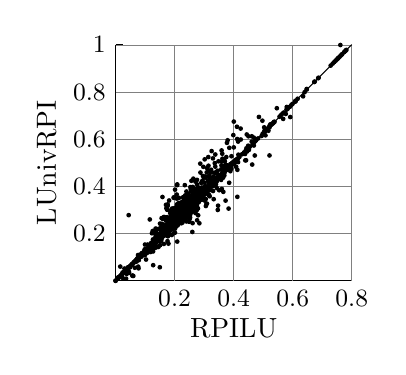
\begin{tikzpicture}

\draw (0,0) -- (3,0);
\node at (1.5,-0.6) {RPILU};
\node [anchor=north] at (0.75,0) {\small 0.2};
\draw (0.75,0) -- (0.75,0.1);
\draw [style=help lines] (0.75,0) -- (0.75,3);
\node [anchor=north] at (1.5,0) {\small 0.4};
\draw (1.5,0) -- (1.5,0.1);
\draw [style=help lines] (1.5,0) -- (1.5,3);
\node [anchor=north] at (2.25,0) {\small 0.6};
\draw (2.25,0) -- (2.25,0.1);
\draw [style=help lines] (2.25,0) -- (2.25,3);
\node [anchor=north] at (3,0) {\small 0.8};
\draw (3,0) -- (3,0.1);
\draw [style=help lines] (3,0) -- (3,3);
\draw (0,0) -- (0,3);
\node [rotate=90] at (-2.5em,1.5) {LUnivRPI};
\node [anchor=east] at (0,0.599) {\small 0.2};
\draw (0,0.599) -- (0.1,0.599);
\draw [style=help lines] (0,0.599) -- (3,0.599);
\node [anchor=east] at (0,1.198) {\small 0.4};
\draw (0,1.198) -- (0.1,1.198);
\draw [style=help lines] (0,1.198) -- (3,1.198);
\node [anchor=east] at (0,1.797) {\small 0.6};
\draw (0,1.797) -- (0.1,1.797);
\draw [style=help lines] (0,1.797) -- (3,1.797);
\node [anchor=east] at (0,2.396) {\small 0.8};
\draw (0,2.396) -- (0.1,2.396);
\draw [style=help lines] (0,2.396) -- (3,2.396);
\node [anchor=east] at (0,2.995) {\small 1};
\draw (0,2.995) -- (0.1,2.995);
\draw [style=help lines] (0,2.995) -- (3,2.995);
\foreach \pos in {
	(0.000000, 0.000000),
	(0.022556, 0.022556),
	(0.028846, 0.028846),
	(0.034884, 0.034884),
	(0.034575, 0.044224),
	(0.039735, 0.039735),
	(0.047782, 0.047782),
	(0.055046, 0.055046),
	(0.063559, 0.063559),
	(0.089300, 0.036203),
	(0.068354, 0.068354),
	(0.075949, 0.075949),
	(0.083333, 0.083333),
	(0.088235, 0.088235),
	(0.092593, 0.092593),
	(0.134328, 0.026866),
	(0.090106, 0.106007),
	(0.099919, 0.099919),
	(0.104167, 0.104167),
	(0.110092, 0.110092),
	(0.114504, 0.114504),
	(0.142105, 0.086842),
	(0.122041, 0.122041),
	(0.128571, 0.128571),
	(0.060000, 0.180000),
	(0.113402, 0.154639),
	(0.136364, 0.136364),
	(0.172727, 0.100000),
	(0.142012, 0.142012),
	(0.169014, 0.118310),
	(0.146341, 0.146341),
	(0.147337, 0.153550),
	(0.153846, 0.153846),
	(0.213198, 0.065990),
	(0.218182, 0.062338),
	(0.160714, 0.160714),
	(0.155592, 0.170178),
	(0.225606, 0.061529),
	(0.166667, 0.166667),
	(0.173077, 0.173077),
	(0.183406, 0.170306),
	(0.177515, 0.177515),
	(0.182657, 0.182657),
	(0.190909, 0.190909),
	(0.195918, 0.195918),
	(0.204545, 0.204545),
	(0.244616, 0.164959),
	(0.209031, 0.210782),
	(0.214286, 0.214286),
	(0.223520, 0.221549),
	(0.230207, 0.230207),
	(0.292018, 0.157629),
	(0.234894, 0.234919),
	(0.239276, 0.239276),
	(0.287671, 0.179795),
	(0.243542, 0.243542),
	(0.248894, 0.248894),
	(0.255783, 0.252513),
	(0.266199, 0.242723),
	(0.258846, 0.258572),
	(0.270626, 0.257542),
	(0.265200, 0.263854),
	(0.269181, 0.268379),
	(0.275291, 0.268163),
	(0.275252, 0.274993),
	(0.273399, 0.280788),
	(0.295549, 0.261387),
	(0.282602, 0.276229),
	(0.284035, 0.282957),
	(0.288462, 0.288462),
	(0.293995, 0.293995),
	(0.298913, 0.298913),
	(0.306519, 0.295294),
	(0.304424, 0.302453),
	(0.293392, 0.314537),
	(0.285714, 0.326531),
	(0.309164, 0.307831),
	(0.317048, 0.308260),
	(0.313453, 0.313349),
	(0.306996, 0.320919),
	(0.320741, 0.313489),
	(0.330679, 0.306296),
	(0.317708, 0.322917),
	(0.326093, 0.316872),
	(0.323818, 0.323818),
	(0.315600, 0.333600),
	(0.328222, 0.327992),
	(0.332547, 0.332547),
	(0.387818, 0.269324),
	(0.339851, 0.333402),
	(0.339416, 0.339416),
	(0.345858, 0.338856),
	(0.354665, 0.330206),
	(0.334023, 0.351093),
	(0.344828, 0.344828),
	(0.372407, 0.323912),
	(0.351436, 0.348536),
	(0.358391, 0.348831),
	(0.355078, 0.354582),
	(0.364317, 0.352429),
	(0.361225, 0.358971),
	(0.380669, 0.341907),
	(0.371588, 0.352141),
	(0.364419, 0.364419),
	(0.370711, 0.360210),
	(0.478022, 0.197802),
	(0.369200, 0.368275),
	(0.375389, 0.365496),
	(0.382118, 0.362346),
	(0.387746, 0.357339),
	(0.373937, 0.372400),
	(0.381738, 0.371255),
	(0.367742, 0.387097),
	(0.378076, 0.377479),
	(0.388171, 0.369689),
	(0.398700, 0.360268),
	(0.384296, 0.378654),
	(0.376535, 0.388813),
	(0.407384, 0.357285),
	(0.393284, 0.376351),
	(0.385410, 0.384763),
	(0.371429, 0.400000),
	(0.401309, 0.370806),
	(0.389312, 0.389461),
	(0.398151, 0.384707),
	(0.395520, 0.393123),
	(0.401035, 0.390751),
	(0.413198, 0.380177),
	(0.400984, 0.397114),
	(0.408824, 0.390137),
	(0.398674, 0.406416),
	(0.407415, 0.398638),
	(0.404830, 0.404830),
	(0.413967, 0.396898),
	(0.419955, 0.392862),
	(0.411514, 0.403804),
	(0.447395, 0.365598),
	(0.409902, 0.409648),
	(0.419624, 0.402414),
	(0.414543, 0.414197),
	(0.419741, 0.409620),
	(0.562500, 0.171655),
	(0.441445, 0.392429),
	(0.420526, 0.415948),
	(0.374026, 0.459740),
	(0.426119, 0.413636),
	(0.440829, 0.401792),
	(0.422182, 0.422182),
	(0.436796, 0.408040),
	(0.433435, 0.415817),
	(0.450180, 0.401541),
	(0.427987, 0.425591),
	(0.477465, 0.372692),
	(0.436370, 0.422848),
	(0.431995, 0.430569),
	(0.424779, 0.438053),
	(0.409938, 0.459627),
	(0.437492, 0.434122),
	(0.447635, 0.427734),
	(0.439649, 0.440233),
	(0.455157, 0.424541),
	(0.445404, 0.435769),
	(0.444396, 0.444186),
	(0.463486, 0.426417),
	(0.452253, 0.442553),
	(0.461794, 0.433555),
	(0.449267, 0.449064),
	(0.485346, 0.411489),
	(0.474719, 0.425292),
	(0.458161, 0.446142),
	(0.454311, 0.453054),
	(0.469972, 0.443377),
	(0.457098, 0.458545),
	(0.463736, 0.454544),
	(0.462545, 0.462013),
	(0.486281, 0.437290),
	(0.468771, 0.460270),
	(0.466904, 0.466452),
	(0.452772, 0.480493),
	(0.512121, 0.421212),
	(0.480412, 0.459803),
	(0.473684, 0.466744),
	(0.489568, 0.453800),
	(0.471805, 0.472556),
	(0.469036, 0.478173),
	(0.478968, 0.471520),
	(0.483933, 0.467733),
	(0.477878, 0.477517),
	(0.503753, 0.452990),
	(0.491125, 0.469236),
	(0.484051, 0.476676),
	(0.481577, 0.483140),
	(0.501044, 0.467243),
	(0.489833, 0.481374),
	(0.487049, 0.487049),
	(0.497297, 0.481081),
	(0.484709, 0.497208),
	(0.545670, 0.429860),
	(0.495726, 0.486985),
	(0.492373, 0.492132),
	(0.508184, 0.478660),
	(0.503059, 0.486929),
	(0.499177, 0.492046),
	(0.496330, 0.499698),
	(0.514779, 0.481489),
	(0.508778, 0.489682),
	(0.474820, 0.524333),
	(0.504151, 0.497453),
	(0.486376, 0.514986),
	(0.501155, 0.503464),
	(0.513560, 0.498033),
	(0.508215, 0.503762),
	(0.520594, 0.497793),
	(0.508507, 0.510155),
	(0.515061, 0.507594),
	(0.565949, 0.452323),
	(0.515260, 0.514173),
	(0.523865, 0.510974),
	(0.520529, 0.517464),
	(0.515702, 0.525620),
	(0.530049, 0.511960),
	(0.521934, 0.523352),
	(0.527823, 0.518504),
	(0.539892, 0.507499),
	(0.516432, 0.533646),
	(0.504505, 0.547297),
	(0.527733, 0.525370),
	(0.539118, 0.519203),
	(0.525401, 0.533422),
	(0.531032, 0.530958),
	(0.546039, 0.517131),
	(0.538117, 0.525696),
	(0.522737, 0.542180),
	(0.556681, 0.510249),
	(0.535479, 0.535069),
	(0.462295, 0.603279),
	(0.542719, 0.535296),
	(0.534743, 0.543807),
	(0.549745, 0.531888),
	(0.543023, 0.542350),
	(0.577982, 0.506422),
	(0.564838, 0.523691),
	(0.614284, 0.467686),
	(0.550083, 0.541852),
	(0.543210, 0.549383),
	(0.508541, 0.583443),
	(0.556675, 0.538924),
	(0.575860, 0.522055),
	(0.551209, 0.548425),
	(0.582329, 0.524096),
	(0.560810, 0.547419),
	(0.556385, 0.552888),
	(0.544983, 0.564446),
	(0.502392, 0.602871),
	(0.579525, 0.531454),
	(0.567796, 0.544318),
	(0.574570, 0.537508),
	(0.471406, 0.631404),
	(0.531310, 0.582785),
	(0.559181, 0.559023),
	(0.488716, 0.622150),
	(0.565231, 0.553924),
	(0.580072, 0.541226),
	(0.557851, 0.566116),
	(0.565781, 0.560014),
	(0.557138, 0.574966),
	(0.566820, 0.566820),
	(0.529631, 0.602062),
	(0.573043, 0.566530),
	(0.501548, 0.631579),
	(0.570624, 0.572528),
	(0.588620, 0.554731),
	(0.567413, 0.578345),
	(0.579177, 0.567443),
	(0.576972, 0.574719),
	(0.583475, 0.572571),
	(0.592996, 0.562925),
	(0.563269, 0.593023),
	(0.513793, 0.636782),
	(0.573937, 0.585028),
	(0.672091, 0.471023),
	(0.581099, 0.580736),
	(0.588298, 0.577660),
	(0.603705, 0.563366),
	(0.585803, 0.585508),
	(0.659864, 0.503401),
	(0.574521, 0.599500),
	(0.596143, 0.578609),
	(0.583853, 0.591965),
	(0.602125, 0.575303),
	(0.591766, 0.588407),
	(0.508619, 0.662460),
	(0.518575, 0.657316),
	(0.587852, 0.597674),
	(0.604636, 0.582716),
	(0.613559, 0.574295),
	(0.593662, 0.594899),
	(0.578804, 0.611413),
	(0.602496, 0.591150),
	(0.600292, 0.598104),
	(0.166667, 0.833333),
	(0.597716, 0.605203),
	(0.615015, 0.591258),
	(0.605821, 0.602861),
	(0.611465, 0.597568),
	(0.625467, 0.584720),
	(0.602334, 0.609515),
	(0.550435, 0.660000),
	(0.579055, 0.635736),
	(0.631521, 0.583657),
	(0.610072, 0.607405),
	(0.619847, 0.597584),
	(0.615578, 0.602921),
	(0.625418, 0.593831),
	(0.607038, 0.615836),
	(0.648491, 0.573515),
	(0.613324, 0.613108),
	(0.626006, 0.601090),
	(0.618817, 0.608803),
	(0.591671, 0.636784),
	(0.613293, 0.619335),
	(0.625509, 0.608141),
	(0.576528, 0.655027),
	(0.665525, 0.564847),
	(0.633271, 0.601128),
	(0.619438, 0.617937),
	(0.609499, 0.630607),
	(0.618232, 0.624997),
	(0.635533, 0.609698),
	(0.642222, 0.603370),
	(0.624464, 0.622049),
	(0.604396, 0.645604),
	(0.630861, 0.620307),
	(0.615142, 0.636435),
	(0.667263, 0.583184),
	(0.643003, 0.610247),
	(0.625220, 0.628517),
	(0.649956, 0.603342),
	(0.579172, 0.671915),
	(0.641497, 0.616339),
	(0.631784, 0.626505),
	(0.435311, 0.778413),
	(0.637720, 0.624364),
	(0.632758, 0.632715),
	(0.615000, 0.650000),
	(0.656665, 0.607969),
	(0.646214, 0.622715),
	(0.611448, 0.660885),
	(0.637621, 0.638473),
	(0.655465, 0.620936),
	(0.584448, 0.689799),
	(0.606099, 0.670902),
	(0.629898, 0.648786),
	(0.648649, 0.632883),
	(0.636640, 0.645105),
	(0.643870, 0.638600),
	(0.677656, 0.604396),
	(0.642729, 0.646315),
	(0.657056, 0.634599),
	(0.648718, 0.643280),
	(0.617414, 0.675462),
	(0.635745, 0.658723),
	(0.642785, 0.652868),
	(0.624677, 0.671080),
	(0.655901, 0.641987),
	(0.649135, 0.649906),
	(0.614597, 0.683739),
	(0.564516, 0.725806),
	(0.666000, 0.636000),
	(0.714599, 0.581229),
	(0.646637, 0.658214),
	(0.663366, 0.641516),
	(0.636181, 0.669347),
	(0.658168, 0.648170),
	(0.603910, 0.699890),
	(0.642609, 0.664608),
	(0.654825, 0.653205),
	(0.783251, 0.497537),
	(0.632342, 0.679182),
	(0.627804, 0.684300),
	(0.666932, 0.647012),
	(0.661601, 0.653419),
	(0.654640, 0.661359),
	(0.611856, 0.701699),
	(0.686222, 0.630130),
	(0.589047, 0.722834),
	(0.650054, 0.669556),
	(0.645228, 0.674274),
	(0.669706, 0.653207),
	(0.685345, 0.637315),
	(0.661832, 0.661832),
	(0.675270, 0.650060),
	(0.683120, 0.644765),
	(0.631579, 0.696026),
	(0.614787, 0.711224),
	(0.668191, 0.661332),
	(0.660642, 0.671048),
	(0.653303, 0.680638),
	(0.667712, 0.667712),
	(0.679142, 0.656550),
	(0.673727, 0.664376),
	(0.697674, 0.641139),
	(0.662371, 0.677835),
	(0.655275, 0.686478),
	(0.690801, 0.652470),
	(0.680974, 0.663630),
	(0.670270, 0.675676),
	(0.636464, 0.707735),
	(0.674736, 0.671528),
	(0.687664, 0.664042),
	(0.681655, 0.670863),
	(0.669454, 0.684095),
	(0.677905, 0.676972),
	(0.695131, 0.662172),
	(0.657919, 0.700094),
	(0.745701, 0.607429),
	(0.679876, 0.684211),
	(0.691349, 0.672988),
	(0.685007, 0.680992),
	(0.698696, 0.669809),
	(0.666377, 0.702867),
	(0.680531, 0.690265),
	(0.754568, 0.610833),
	(0.692145, 0.681382),
	(0.686452, 0.688050),
	(0.719727, 0.654123),
	(0.661905, 0.714286),
	(0.676278, 0.701955),
	(0.656997, 0.720137),
	(0.709167, 0.669167),
	(0.714153, 0.665766),
	(0.687423, 0.694356),
	(0.702323, 0.679633),
	(0.694732, 0.687820),
	(0.674586, 0.711498),
	(0.693909, 0.693909),
	(0.701768, 0.685972),
	(0.666436, 0.722491),
	(0.699736, 0.691677),
	(0.689532, 0.702317),
	(0.672750, 0.719469),
	(0.708753, 0.685584),
	(0.585000, 0.795000),
	(0.695503, 0.700590),
	(0.715607, 0.681605),
	(0.601744, 0.784884),
	(0.707358, 0.692308),
	(0.702706, 0.699210),
	(0.691631, 0.710638),
	(0.726631, 0.680217),
	(0.702036, 0.706324),
	(0.720594, 0.688403),
	(0.691031, 0.718293),
	(0.685828, 0.723974),
	(0.640477, 0.764626),
	(0.709139, 0.703866),
	(0.741212, 0.673968),
	(0.692557, 0.724919),
	(0.705156, 0.713212),
	(0.642857, 0.772321),
	(0.608932, 0.799564),
	(0.756164, 0.662100),
	(0.689826, 0.731079),
	(0.711353, 0.710480),
	(0.723788, 0.698083),
	(0.716995, 0.705947),
	(0.742160, 0.681343),
	(0.679403, 0.744086),
	(0.711391, 0.716801),
	(0.703796, 0.726198),
	(0.695364, 0.735099),
	(0.717713, 0.713518),
	(0.691437, 0.741162),
	(0.750228, 0.681715),
	(0.732464, 0.701654),
	(0.727200, 0.708476),
	(0.713470, 0.722720),
	(0.703447, 0.732583),
	(0.615471, 0.810538),
	(0.739053, 0.699732),
	(0.720661, 0.718893),
	(0.759462, 0.678722),
	(0.710632, 0.732538),
	(0.719154, 0.727382),
	(0.730190, 0.716726),
	(0.727979, 0.722531),
	(0.639756, 0.801980),
	(0.750124, 0.700708),
	(0.653998, 0.793416),
	(0.724649, 0.730079),
	(0.741538, 0.713096),
	(0.764197, 0.689562),
	(0.721056, 0.734896),
	(0.738292, 0.719008),
	(0.707555, 0.750934),
	(0.730655, 0.729710),
	(0.737341, 0.728187),
	(0.748077, 0.717559),
	(0.744422, 0.723124),
	(0.718587, 0.749042),
	(0.706656, 0.760464),
	(0.731223, 0.736893),
	(0.770504, 0.695778),
	(0.727116, 0.742152),
	(0.656402, 0.807131),
	(0.757036, 0.714581),
	(0.743611, 0.729581),
	(0.739785, 0.734409),
	(0.751145, 0.723593),
	(0.736811, 0.739889),
	(0.729795, 0.747679),
	(0.679455, 0.794554),
	(0.723061, 0.755287),
	(0.749541, 0.730934),
	(0.693407, 0.784870),
	(0.719430, 0.762805),
	(0.711588, 0.770166),
	(0.736728, 0.746166),
	(0.745416, 0.737740),
	(0.780930, 0.701970),
	(0.762513, 0.725240),
	(0.745487, 0.744585),
	(0.756898, 0.735490),
	(0.751768, 0.741603),
	(0.789564, 0.704061),
	(0.740817, 0.756337),
	(0.721226, 0.775403),
	(0.734307, 0.763916),
	(0.763417, 0.735329),
	(0.751237, 0.748598),
	(0.757756, 0.742930),
	(0.747274, 0.753587),
	(0.776899, 0.723892),
	(0.756920, 0.750622),
	(0.773604, 0.734224),
	(0.735504, 0.772818),
	(0.751733, 0.758256),
	(0.765514, 0.745164),
	(0.723367, 0.786867),
	(0.745988, 0.766667),
	(0.780892, 0.731121),
	(0.791336, 0.719819),
	(0.758847, 0.756881),
	(0.752684, 0.764985),
	(0.774810, 0.742662),
	(0.769972, 0.749387),
	(0.765130, 0.755043),
	(0.760112, 0.763165),
	(0.788860, 0.733959),
	(0.782496, 0.740901),
	(0.752401, 0.771689),
	(0.729960, 0.795848),
	(0.766390, 0.762416),
	(0.760481, 0.771571),
	(0.786157, 0.746549),
	(0.778025, 0.756397),
	(0.766846, 0.769317),
	(0.775025, 0.761776),
	(0.755313, 0.782041),
	(0.723266, 0.811805),
	(0.717493, 0.816971),
	(0.798344, 0.738927),
	(0.705698, 0.829587),
	(0.792930, 0.749359),
	(0.783383, 0.760723),
	(0.773640, 0.770817),
	(0.810154, 0.732769),
	(0.743241, 0.801787),
	(0.770451, 0.776401),
	(0.739398, 0.806589),
	(0.761697, 0.786026),
	(0.756048, 0.792339),
	(0.779754, 0.769295),
	(0.753434, 0.798561),
	(0.776904, 0.776904),
	(0.773205, 0.781766),
	(0.763525, 0.793033),
	(0.789676, 0.767214),
	(0.812655, 0.743176),
	(0.785739, 0.774261),
	(0.695438, 0.856350),
	(0.715630, 0.840574),
	(0.737750, 0.822142),
	(0.802239, 0.759595),
	(0.748544, 0.812621),
	(0.779727, 0.783827),
	(0.727506, 0.833901),
	(0.785145, 0.780264),
	(0.835025, 0.730080),
	(0.777257, 0.791325),
	(0.797771, 0.771497),
	(0.748385, 0.820237),
	(0.792832, 0.777591),
	(0.762066, 0.807790),
	(0.827545, 0.742444),
	(0.774128, 0.798694),
	(0.786585, 0.786585),
	(0.715026, 0.854922),
	(0.655539, 0.901366),
	(0.792627, 0.784346),
	(0.808010, 0.769489),
	(0.801678, 0.776149),
	(0.752890, 0.824387),
	(0.814012, 0.764387),
	(0.782642, 0.797149),
	(0.775382, 0.805242),
	(0.791667, 0.791667),
	(0.799166, 0.784863),
	(0.766423, 0.817518),
	(0.789440, 0.797977),
	(0.806281, 0.782423),
	(0.817593, 0.770642),
	(0.686636, 0.889401),
	(0.829037, 0.759074),
	(0.797893, 0.792146),
	(0.645472, 0.921002),
	(0.849036, 0.737723),
	(0.725580, 0.860251),
	(0.796321, 0.798328),
	(0.812322, 0.782938),
	(0.759069, 0.834783),
	(0.788613, 0.807126),
	(0.826341, 0.768735),
	(0.806818, 0.789367),
	(0.778626, 0.817381),
	(0.765501, 0.829889),
	(0.750887, 0.845244),
	(0.745050, 0.851485),
	(0.820836, 0.779622),
	(0.804204, 0.798157),
	(0.798184, 0.804469),
	(0.783590, 0.821211),
	(0.818930, 0.787380),
	(0.811644, 0.795205),
	(0.805132, 0.805132),
	(0.833818, 0.776775),
	(0.795670, 0.817321),
	(0.780034, 0.832610),
	(0.813221, 0.801160),
	(0.843103, 0.770690),
	(0.801751, 0.813846),
	(0.792855, 0.823470),
	(0.788285, 0.828452),
	(0.775347, 0.841624),
	(0.809524, 0.809524),
	(0.820085, 0.799434),
	(0.828054, 0.792479),
	(0.818228, 0.805152),
	(0.808021, 0.816072),
	(0.800772, 0.823262),
	(0.842713, 0.780782),
	(0.826793, 0.799203),
	(0.797583, 0.828399),
	(0.773913, 0.851304),
	(0.814186, 0.813686),
	(0.743192, 0.879349),
	(0.850427, 0.776353),
	(0.760956, 0.864542),
	(0.834929, 0.794649),
	(0.820432, 0.810968),
	(0.794891, 0.836066),
	(0.975494, 0.619971),
	(0.817452, 0.818790),
	(0.844299, 0.791078),
	(0.640449, 0.963884),
	(0.662148, 0.950108),
	(0.812898, 0.825043),
	(0.836738, 0.801512),
	(0.796970, 0.843939),
	(0.810100, 0.831380),
	(0.843112, 0.798970),
	(0.850365, 0.792492),
	(0.827428, 0.817303),
	(0.836507, 0.809945),
	(0.819021, 0.828255),
	(0.718232, 0.917127),
	(0.861770, 0.785027),
	(0.796702, 0.852804),
	(0.850848, 0.799164),
	(0.826141, 0.825324),
	(0.831631, 0.822581),
	(0.847308, 0.806921),
	(0.730435, 0.914907),
	(0.823985, 0.832689),
	(0.898413, 0.753305),
	(0.780466, 0.875694),
	(0.830623, 0.829760),
	(0.662136, 0.969903),
	(0.818344, 0.842386),
	(0.844961, 0.817829),
	(0.850781, 0.813281),
	(0.809772, 0.854244),
	(0.885005, 0.776089),
	(0.826014, 0.839038),
	(0.841188, 0.823863),
	(0.837138, 0.828632),
	(0.816191, 0.849370),
	(0.857408, 0.809568),
	(0.831954, 0.835773),
	(0.863090, 0.806072),
	(0.786822, 0.880976),
	(0.799062, 0.871212),
	(0.825656, 0.847522),
	(0.849943, 0.823979),
	(0.843788, 0.830533),
	(0.837669, 0.837669),
	(0.813369, 0.861497),
	(0.876133, 0.798557),
	(0.869807, 0.807593),
	(0.834846, 0.844571),
	(0.847044, 0.837731),
	(0.792668, 0.891277),
	(0.843613, 0.843613),
	(0.839437, 0.849106),
	(0.869737, 0.819211),
	(0.875905, 0.812621),
	(0.829018, 0.861318),
	(0.858629, 0.831825),
	(0.854385, 0.836311),
	(0.756027, 0.926712),
	(0.835309, 0.857018),
	(0.933714, 0.749159),
	(0.850414, 0.844408),
	(0.846727, 0.849792),
	(0.876486, 0.819098),
	(0.888205, 0.808622),
	(0.857384, 0.842165),
	(0.843603, 0.857675),
	(0.831642, 0.870304),
	(0.855145, 0.848306),
	(0.868207, 0.836413),
	(0.851999, 0.854148),
	(0.882779, 0.822508),
	(0.864108, 0.842253),
	(0.889535, 0.816661),
	(0.817490, 0.889734),
	(0.900790, 0.806429),
	(0.895844, 0.813203),
	(0.830192, 0.881616),
	(0.836333, 0.875889),
	(0.870536, 0.842174),
	(0.858634, 0.854719),
	(0.863702, 0.850169),
	(0.810302, 0.904523),
	(0.910644, 0.803767),
	(0.849268, 0.869078),
	(0.858637, 0.860825),
	(0.854866, 0.865772),
	(0.885289, 0.835371),
	(0.866699, 0.855863),
	(0.938965, 0.776367),
	(0.596084, 1.063814),
	(0.844833, 0.879440),
	(0.893392, 0.833350),
	(0.978592, 0.731627),
	(0.864238, 0.864238),
	(0.852905, 0.876391),
	(0.798065, 0.926844),
	(0.857468, 0.872252),
	(0.881662, 0.847948),
	(0.872633, 0.857955),
	(0.680372, 1.019395),
	(0.838347, 0.894879),
	(0.871533, 0.864964),
	(0.866335, 0.870532),
	(0.882401, 0.854699),
	(0.878661, 0.860571),
	(0.808989, 0.926966),
	(0.897534, 0.843135),
	(0.905539, 0.834985),
	(0.862741, 0.879927),
	(0.876899, 0.867994),
	(0.869136, 0.876543),
	(0.856620, 0.889567),
	(0.892351, 0.856306),
	(0.907303, 0.840875),
	(0.850642, 0.899650),
	(0.876719, 0.875246),
	(0.884234, 0.868617),
	(0.946985, 0.803116),
	(0.874558, 0.881625),
	(0.845300, 0.911932),
	(0.896487, 0.862763),
	(0.882678, 0.877150),
	(0.860104, 0.899827),
	(0.917439, 0.841618),
	(0.852154, 0.907903),
	(0.780932, 0.969881),
	(0.902745, 0.858014),
	(0.888672, 0.872678),
	(0.880251, 0.884013),
	(0.870641, 0.895388),
	(0.876223, 0.889961),
	(0.790432, 0.967155),
	(0.895791, 0.870535),
	(0.832646, 0.932528),
	(0.889049, 0.879202),
	(0.904517, 0.864105),
	(0.923239, 0.846010),
	(0.914771, 0.856342),
	(0.853571, 0.917857),
	(0.895878, 0.876753),
	(0.931742, 0.839030),
	(0.887139, 0.886483),
	(0.865290, 0.908831),
	(0.879188, 0.895939),
	(0.819048, 0.952381),
	(0.828105, 0.948557),
	(0.904780, 0.875744),
	(0.945968, 0.833749),
	(0.867544, 0.915443),
	(0.891062, 0.892795),
	(0.901083, 0.883452),
	(0.886403, 0.902159),
	(0.897638, 0.892120),
	(0.909774, 0.879854),
	(0.881337, 0.908468),
	(0.893154, 0.899167),
	(0.903714, 0.889180),
	(0.930990, 0.861612),
	(0.799509, 0.986088),
	(0.877256, 0.918412),
	(0.887551, 0.909408),
	(0.902232, 0.896022),
	(0.919030, 0.878804),
	(0.867686, 0.930551),
	(0.915789, 0.885764),
	(0.898828, 0.904038),
	(0.938019, 0.866630),
	(0.904591, 0.902349),
	(0.929348, 0.879529),
	(0.897629, 0.912307),
	(0.873987, 0.935151),
	(0.920292, 0.889980),
	(0.910658, 0.902901),
	(0.917594, 0.898211),
	(0.855407, 0.958964),
	(0.936498, 0.880858),
	(0.909643, 0.908929),
	(0.904252, 0.914622),
	(0.737786, 1.054509),
	(0.894432, 0.926162),
	(0.902376, 0.920924),
	(1.036045, 0.768280),
	(0.868816, 0.953706),
	(1.064516, 0.729997),
	(0.910501, 0.915153),
	(0.926009, 0.899973),
	(0.827487, 0.991831),
	(0.880952, 0.946429),
	(0.741940, 1.059448),
	(0.919658, 0.909783),
	(0.935765, 0.893980),
	(0.954003, 0.876189),
	(0.917293, 0.916792),
	(0.844404, 0.984751),
	(0.911868, 0.922679),
	(0.966829, 0.866782),
	(0.935949, 0.901107),
	(0.877078, 0.959079),
	(0.859499, 0.974954),
	(0.923420, 0.917119),
	(0.778462, 1.043077),
	(0.917419, 0.925189),
	(0.907734, 0.936228),
	(0.914832, 0.931034),
	(0.901863, 0.943602),
	(0.936865, 0.909785),
	(0.932373, 0.915686),
	(0.926320, 0.922902),
	(0.953089, 0.896715),
	(0.867151, 0.982356),
	(0.908609, 0.945412),
	(0.902359, 0.951996),
	(0.926317, 0.929044),
	(0.936487, 0.923442),
	(0.942393, 0.917823),
	(0.917621, 0.943050),
	(0.926438, 0.935266),
	(0.954961, 0.906514),
	(0.851064, 1.005319),
	(0.908888, 0.954164),
	(0.935407, 0.932021),
	(0.953567, 0.914685),
	(0.886308, 0.980440),
	(0.941130, 0.928186),
	(0.964264, 0.905042),
	(0.931402, 0.939024),
	(0.947258, 0.924236),
	(0.984297, 0.885399),
	(0.904551, 0.967971),
	(0.915227, 0.958005),
	(0.805046, 1.052752),
	(0.870377, 1.000718),
	(0.938190, 0.937638),
	(0.927492, 0.948640),
	(0.953397, 0.925110),
	(0.917024, 0.964235),
	(1.016660, 0.858571),
	(0.935866, 0.946139),
	(0.959478, 0.924546),
	(0.942213, 0.942308),
	(0.913968, 0.970043),
	(0.966144, 0.919806),
	(0.951913, 0.934930),
	(0.935025, 0.953735),
	(0.910714, 0.977303),
	(0.949007, 0.941974),
	(0.876581, 1.011339),
	(1.049268, 0.831425),
	(0.945182, 0.949036),
	(0.923561, 0.972363),
	(0.884116, 1.008492),
	(0.969191, 0.927155),
	(0.777090, 1.094943),
	(0.951258, 0.949161),
	(0.963664, 0.936993),
	(0.894031, 1.003702),
	(0.946739, 0.954917),
	(0.942331, 0.959465),
	(0.959022, 0.944151),
	(0.921077, 0.985401),
	(0.974480, 0.934732),
	(0.943629, 0.966023),
	(0.953039, 0.956864),
	(0.957731, 0.952306),
	(0.912752, 0.997763),
	(0.966374, 0.946380),
	(0.971646, 0.942250),
	(0.952047, 0.964170),
	(0.963771, 0.952655),
	(0.978206, 0.942163),
	(0.961394, 0.960881),
	(0.944439, 0.979488),
	(0.868849, 1.047563),
	(0.858491, 1.056604),
	(0.959520, 0.966623),
	(0.912064, 1.012113),
	(0.967930, 0.959913),
	(0.978773, 0.949038),
	(0.973801, 0.954263),
	(1.005386, 0.921005),
	(0.954717, 0.975300),
	(0.988740, 0.941317),
	(1.031729, 0.897326),
	(0.860929, 1.062904),
	(0.968578, 0.966693),
	(0.974616, 0.960876),
	(0.962930, 0.972785),
	(0.940284, 0.995261),
	(0.982259, 0.959432),
	(0.972012, 0.971622),
	(0.963698, 0.980202),
	(1.005230, 0.938542),
	(0.977761, 0.967961),
	(0.990472, 0.957124),
	(1.002850, 0.944218),
	(0.969974, 0.978543),
	(0.943434, 1.006061),
	(1.012690, 0.936548),
	(0.955972, 0.996108),
	(0.977625, 0.975877),
	(0.989711, 0.963724),
	(0.755824, 1.156857),
	(0.902839, 1.046414),
	(0.957053, 1.003469),
	(1.006866, 0.954846),
	(0.985677, 0.976907),
	(0.977905, 0.986097),
	(0.921896, 1.039591),
	(1.003944, 0.963380),
	(0.993660, 0.974640),
	(1.046829, 0.917936),
	(1.038866, 0.927823),
	(0.977230, 0.993359),
	(0.984964, 0.986277),
	(1.014085, 0.959539),
	(0.994076, 0.983470),
	(0.951340, 1.025150),
	(0.985279, 0.992893),
	(0.884826, 1.084095),
	(0.977944, 1.002289),
	(0.911830, 1.064688),
	(1.012946, 0.969209),
	(0.973648, 1.009096),
	(1.020580, 0.963517),
	(0.941653, 1.042139),
	(0.947906, 1.036613),
	(0.998468, 0.988179),
	(1.011078, 0.977324),
	(0.980429, 1.008388),
	(0.995401, 0.994379),
	(0.902603, 1.079490),
	(0.916307, 1.069543),
	(0.929524, 1.058189),
	(0.967981, 1.024694),
	(1.007210, 0.987607),
	(0.960949, 1.033354),
	(0.994960, 1.000775),
	(1.020066, 0.975192),
	(1.033137, 0.962527),
	(0.977804, 1.019264),
	(1.002887, 0.994670),
	(0.948931, 1.047469),
	(1.017134, 0.982880),
	(0.990729, 1.011281),
	(0.995803, 1.007495),
	(0.977811, 1.026282),
	(1.002803, 1.002586),
	(1.025228, 0.984083),
	(1.011309, 1.000606),
	(1.007440, 1.006613),
	(0.989917, 1.025460),
	(0.994538, 1.021549),
	(1.004801, 1.012321),
	(1.020561, 0.998131),
	(0.924413, 1.087845),
	(0.962345, 1.055291),
	(1.016087, 1.005432),
	(1.002201, 1.022014),
	(1.026705, 0.997471),
	(1.011689, 1.013680),
	(0.983035, 1.043887),
	(1.038594, 0.990801),
	(1.022754, 1.007186),
	(1.014350, 1.020269),
	(0.925102, 1.101931),
	(1.006697, 1.029618),
	(1.032721, 1.005741),
	(0.781395, 1.213953),
	(1.016566, 1.026263),
	(1.045652, 0.998402),
	(1.039030, 1.005752),
	(1.032906, 1.012324),
	(0.959367, 1.083641),
	(0.900196, 1.133580),
	(1.027167, 1.020297),
	(1.008410, 1.039535),
	(1.056832, 0.997205),
	(1.027604, 1.027604),
	(0.784158, 1.223762),
	(1.019690, 1.036672),
	(1.042208, 1.015422),
	(1.037290, 1.020452),
	(0.985150, 1.074251),
	(1.035623, 1.026955),
	(0.980671, 1.080101),
	(1.027672, 1.037360),
	(1.033701, 1.032756),
	(1.048043, 1.020875),
	(1.060339, 1.010037),
	(1.027780, 1.043378),
	(1.041736, 1.034725),
	(1.026266, 1.051058),
	(0.984796, 1.090229),
	(1.037809, 1.040895),
	(1.059521, 1.025451),
	(1.046367, 1.039100),
	(1.021963, 1.065716),
	(1.043165, 1.045564),
	(0.984356, 1.102574),
	(1.052583, 1.040129),
	(1.014286, 1.078125),
	(1.070118, 1.023529),
	(1.048247, 1.049522),
	(1.038595, 1.059489),
	(0.999782, 1.096430),
	(1.031776, 1.068690),
	(1.045581, 1.055586),
	(1.062660, 1.039258),
	(1.147132, 0.948878),
	(0.962523, 1.138026),
	(1.047671, 1.062539),
	(1.066794, 1.045165),
	(1.056374, 1.058905),
	(1.062950, 1.056355),
	(0.977609, 1.135946),
	(0.879934, 1.214187),
	(1.055407, 1.065589),
	(1.068566, 1.052632),
	(1.090365, 1.031733),
	(1.079200, 1.043574),
	(1.050448, 1.073349),
	(0.955121, 1.162619),
	(1.075812, 1.054553),
	(1.065608, 1.065608),
	(1.040462, 1.090318),
	(0.969112, 1.154440),
	(1.048622, 1.083244),
	(1.101259, 1.032315),
	(1.017183, 1.117377),
	(1.155328, 0.976972),
	(1.074184, 1.066333),
	(1.040359, 1.100149),
	(1.062668, 1.078841),
	(1.070256, 1.071931),
	(1.085480, 1.058666),
	(1.081860, 1.065187),
	(1.160890, 0.979307),
	(1.056362, 1.092229),
	(1.095050, 1.054497),
	(1.070364, 1.080795),
	(1.102555, 1.048337),
	(1.077397, 1.074318),
	(1.026941, 1.122916),
	(1.131139, 1.018882),
	(0.950818, 1.189381),
	(1.113034, 1.039373),
	(0.967894, 1.176977),
	(1.037749, 1.115992),
	(1.088855, 1.066587),
	(1.066224, 1.089365),
	(1.083889, 1.072768),
	(1.053140, 1.103060),
	(1.129739, 1.028174),
	(1.096560, 1.064894),
	(1.080901, 1.080901),
	(1.055921, 1.108553),
	(1.077129, 1.088425),
	(1.088582, 1.077519),
	(1.123512, 1.044261),
	(1.108909, 1.060634),
	(1.034333, 1.134348),
	(0.974684, 1.186709),
	(1.084046, 1.089744),
	(1.091364, 1.086082),
	(0.980943, 1.191575),
	(1.014676, 1.163140),
	(1.098383, 1.084906),
	(1.145827, 1.037675),
	(1.087045, 1.099190),
	(1.113313, 1.073778),
	(1.095591, 1.094213),
	(1.085311, 1.107405),
	(1.100501, 1.098550),
	(1.112153, 1.087650),
	(1.086230, 1.120984),
	(1.100694, 1.107639),
	(1.096237, 1.119396),
	(1.109982, 1.106396),
	(1.097439, 1.125835),
	(1.120908, 1.103676),
	(1.115984, 1.109770),
	(1.134454, 1.096273),
	(1.108549, 1.124032),
	(1.082350, 1.149307),
	(1.298528, 0.899439),
	(1.122930, 1.111139),
	(1.045283, 1.184906),
	(1.105612, 1.129337),
	(1.099692, 1.135663),
	(1.119196, 1.118073),
	(1.130740, 1.106824),
	(1.061292, 1.179986),
	(1.128039, 1.116514),
	(1.136653, 1.107859),
	(1.123624, 1.123942),
	(0.963855, 1.269076),
	(1.120687, 1.134780),
	(1.126802, 1.130195),
	(1.129691, 1.135809),
	(1.036769, 1.222841),
	(1.144306, 1.123488),
	(1.154525, 1.115331),
	(1.195920, 1.072539),
	(1.137031, 1.135458),
	(1.187964, 1.082149),
	(1.093664, 1.183606),
	(1.185439, 1.092415),
	(1.144638, 1.137088),
	(1.302281, 0.953468),
	(1.117200, 1.166722),
	(1.163695, 1.120620),
	(1.130453, 1.154833),
	(1.014583, 1.258333),
	(1.152476, 1.134999),
	(1.140000, 1.150000),
	(1.246615, 1.036088),
	(1.152747, 1.142657),
	(1.146550, 1.148882),
	(1.139928, 1.156574),
	(1.130957, 1.173465),
	(0.988318, 1.296729),
	(1.168521, 1.137043),
	(1.153028, 1.152851),
	(1.120709, 1.185167),
	(1.162643, 1.154172),
	(1.159526, 1.159526),
	(1.130999, 1.187648),
	(1.155479, 1.167466),
	(1.148479, 1.177728),
	(1.034849, 1.281158),
	(1.145148, 1.187249),
	(1.167316, 1.166469),
	(1.088946, 1.243523),
	(1.159404, 1.178616),
	(1.143168, 1.198694),
	(1.174062, 1.171558),
	(1.197578, 1.150874),
	(1.166234, 1.183766),
	(1.173711, 1.177577),
	(1.098513, 1.250000),
	(1.159054, 1.194127),
	(1.164706, 1.191091),
	(1.181774, 1.175988),
	(1.192339, 1.167628),
	(1.182573, 1.184719),
	(1.172253, 1.195509),
	(1.178065, 1.190829),
	(1.190342, 1.184815),
	(1.129749, 1.244508),
	(1.200268, 1.178459),
	(1.238444, 1.140140),
	(1.103516, 1.271484),
	(1.194030, 1.194030),
	(1.186272, 1.207268),
	(1.194319, 1.203166),
	(1.207103, 1.193949),
	(1.435841, 0.916648),
	(1.197446, 1.212346),
	(1.212305, 1.199088),
	(1.210157, 1.210157),
	(1.183099, 1.238353),
	(1.225136, 1.197314),
	(1.190635, 1.234337),
	(1.217028, 1.217028),
	(1.190251, 1.245091),
	(1.125215, 1.309592),
	(1.202442, 1.240116),
	(1.224753, 1.218705),
	(1.238337, 1.205118),
	(1.397624, 1.017896),
	(1.232038, 1.214021),
	(1.172671, 1.273506),
	(1.109126, 1.331650),
	(1.201560, 1.252276),
	(1.246482, 1.207832),
	(1.210578, 1.244665),
	(1.227816, 1.227816),
	(1.232784, 1.223301),
	(1.144089, 1.310965),
	(1.233313, 1.233313),
	(1.287447, 1.177127),
	(1.078030, 1.374384),
	(1.315578, 1.149880),
	(1.231035, 1.242958),
	(1.144879, 1.324124),
	(1.238781, 1.238781),
	(1.244295, 1.234139),
	(1.237974, 1.252401),
	(1.198622, 1.298507),
	(1.275787, 1.226180),
	(1.368596, 1.128993),
	(1.268694, 1.245725),
	(1.239249, 1.275591),
	(1.349509, 1.165525),
	(1.262582, 1.262476),
	(1.189323, 1.338606),
	(1.265415, 1.272126),
	(1.254972, 1.287251),
	(1.157691, 1.376792),
	(1.286745, 1.264595),
	(1.277102, 1.276928),
	(1.241476, 1.323706),
	(1.282375, 1.287532),
	(1.115066, 1.446763),
	(1.291234, 1.292147),
	(1.181159, 1.394203),
	(1.280041, 1.311609),
	(1.076031, 1.487214),
	(1.211951, 1.383555),
	(1.222754, 1.376289),
	(1.303531, 1.303531),
	(1.161605, 1.431670),
	(1.304299, 1.315419),
	(1.310432, 1.309862),
	(1.340122, 1.280847),
	(1.310915, 1.317254),
	(1.213831, 1.409976),
	(1.261043, 1.372918),
	(1.314433, 1.323156),
	(1.337716, 1.300097),
	(1.329128, 1.312098),
	(1.273395, 1.367228),
	(1.322578, 1.319714),
	(1.308176, 1.343815),
	(1.326633, 1.326633),
	(1.342159, 1.311100),
	(1.348711, 1.304504),
	(1.180412, 1.460541),
	(1.547228, 1.065936),
	(1.286185, 1.385123),
	(1.366492, 1.309948),
	(1.339217, 1.338452),
	(1.345076, 1.334134),
	(1.338827, 1.346338),
	(1.352639, 1.338384),
	(1.443027, 1.244519),
	(1.296582, 1.397567),
	(1.346395, 1.353534),
	(1.132280, 1.541633),
	(1.363693, 1.350622),
	(1.381020, 1.335694),
	(1.358798, 1.362090),
	(1.266591, 1.449475),
	(1.379769, 1.359472),
	(1.379802, 1.370334),
	(1.356591, 1.398109),
	(1.379602, 1.377739),
	(1.342177, 1.416285),
	(1.259900, 1.493362),
	(1.177952, 1.571003),
	(1.389168, 1.389047),
	(1.391871, 1.413727),
	(1.236818, 1.554117),
	(1.345186, 1.465742),
	(1.380055, 1.433494),
	(1.412117, 1.408875),
	(1.404695, 1.416993),
	(1.366564, 1.455302),
	(1.420317, 1.409524),
	(1.307241, 1.516634),
	(1.410308, 1.425982),
	(1.458224, 1.391340),
	(1.398478, 1.455142),
	(1.435560, 1.425581),
	(1.344907, 1.514129),
	(1.397770, 1.471375),
	(1.432099, 1.439506),
	(1.440811, 1.440233),
	(1.421943, 1.464520),
	(1.468891, 1.420304),
	(1.266976, 1.603686),
	(1.362281, 1.525040),
	(1.220294, 1.646425),
	(1.387931, 1.514224),
	(1.450662, 1.457387),
	(1.456564, 1.455354),
	(1.357798, 1.549803),
	(1.382758, 1.528378),
	(1.462692, 1.459497),
	(1.466799, 1.464970),
	(1.458469, 1.481672),
	(1.478172, 1.477734),
	(1.547323, 1.408739),
	(1.478777, 1.495085),
	(1.531865, 1.446081),
	(1.355323, 1.612954),
	(1.406478, 1.570410),
	(1.498013, 1.492054),
	(1.509183, 1.487386),
	(1.503409, 1.505404),
	(1.497406, 1.513621),
	(1.346996, 1.654945),
	(1.511306, 1.510523),
	(1.523141, 1.512229),
	(1.530875, 1.511149),
	(1.472189, 1.581065),
	(1.529642, 1.529243),
	(1.527110, 1.535317),
	(1.556802, 1.506849),
	(1.538012, 1.538012),
	(1.544983, 1.544983),
	(1.557435, 1.557435),
	(1.444680, 1.688246),
	(1.573389, 1.572733),
	(1.560165, 1.601374),
	(1.647891, 1.528460),
	(1.415088, 1.751436),
	(1.657716, 1.529879),
	(1.501434, 1.693444),
	(1.606623, 1.606564),
	(1.735704, 1.475503),
	(1.423582, 1.783982),
	(1.644841, 1.610640),
	(1.632543, 1.629820),
	(1.653870, 1.653456),
	(1.670283, 1.642042),
	(1.665806, 1.660579),
	(1.556609, 1.767589),
	(1.671731, 1.665270),
	(1.662612, 1.683074),
	(1.544963, 1.800000),
	(1.693806, 1.661888),
	(1.768181, 1.590661),
	(1.495890, 1.849900),
	(1.590639, 1.793561),
	(1.684474, 1.715235),
	(1.701794, 1.701794),
	(1.706790, 1.706388),
	(1.756824, 1.717297),
	(1.744768, 1.744768),
	(1.728638, 1.766849),
	(1.755382, 1.756413),
	(1.541934, 1.955813),
	(1.687959, 1.834537),
	(1.666767, 1.857796),
	(1.766223, 1.765992),
	(1.588697, 1.932441),
	(1.773655, 1.773655),
	(1.502194, 2.021453),
	(1.955203, 1.591291),
	(1.730370, 1.834640),
	(1.785152, 1.783925),
	(1.779854, 1.790575),
	(1.755213, 1.818250),
	(1.810567, 1.807443),
	(1.855539, 1.838997),
	(1.868804, 1.868556),
	(1.904224, 1.846805),
	(1.890277, 1.901899),
	(1.897379, 1.896212),
	(1.905562, 1.910953),
	(1.887945, 1.948244),
	(1.941713, 1.904999),
	(1.932687, 1.922693),
	(1.940173, 1.941131),
	(1.865014, 2.032478),
	(1.955780, 1.948403),
	(1.820835, 2.080332),
	(1.955892, 1.968298),
	(1.966156, 1.986146),
	(1.978911, 1.980897),
	(1.987261, 1.993111),
	(1.996257, 1.997716),
	(2.004235, 2.003383),
	(2.011581, 2.016846),
	(2.019159, 2.019159),
	(2.082724, 2.082724),
	(2.128778, 2.055398),
	(2.096291, 2.096291),
	(2.107660, 2.110754),
	(2.048547, 2.191131),
	(2.127244, 2.127244),
	(2.135859, 2.135859),
	(2.162073, 2.118826),
	(2.218688, 2.079017),
	(2.170420, 2.172437),
	(2.186389, 2.184267),
	(2.174544, 2.206955),
	(2.215284, 2.210222),
	(2.234410, 2.234410),
	(2.248334, 2.246795),
	(2.281871, 2.274534),
	(2.286710, 2.280101),
	(2.284943, 2.285955),
	(2.312344, 2.311098),
	(2.382145, 2.342246),
	(2.400839, 2.394216),
	(2.427526, 2.427875),
	(2.428310, 2.435646),
	(2.523868, 2.523868),
	(2.529708, 2.529708),
	(2.573387, 2.572063),
	(2.578916, 2.578474),
	(2.732408, 2.732408),
	(2.757845, 2.757845),
	(2.777794, 2.777794),
	(2.794091, 2.794091),
	(2.807822, 2.807822),
	(2.819653, 2.819653),
	(2.825481, 2.825481),
	(2.830657, 2.829625),
	(2.844497, 2.844497),
	(2.858762, 2.858762),
	(2.870029, 2.870029),
	(2.879296, 2.879296),
	(2.903025, 2.903025),
	(2.916072, 2.916072),
	(2.925152, 2.925152),
	(2.855262, 2.993609),
	(2.931903, 2.931903),
} \fill \pos circle(0.03);
\draw (0,0) -- (3, 3);
\end{tikzpicture}

  }
  \caption{Comparison of orders to combine {\RPI} and {\LowerUnits}/{\LowerUnivalents}}
  \label{fig:order}
\end{figure}

\end{figure}

\section{Conclusions}

\bibliographystyle{splncs}
\bibliography{../biblio}

\end{document}
